\documentclass[11pt]{article}
\usepackage[T1]{fontenc}
\usepackage[utf8]{inputenc}
\usepackage[margin=1in]{geometry}
\usepackage{amsmath,amssymb}
\usepackage{booktabs}
\usepackage{graphicx}
\usepackage{placeins}
\usepackage{tikz}
\usetikzlibrary{arrows.meta,positioning}
\usepackage[colorlinks=true,linkcolor=blue,citecolor=blue,urlcolor=blue]{hyperref}

\newcommand{\Bdom}{\mathcal{B}}
\newcommand{\Pdom}{\mathcal{P}}
\newcommand{\Sset}{\mathcal{S}}

\begin{document}

\section{PAO domain background}
\label{sec:domain-construction}

The conventional projected-atomic-orbital (PAO) hierarchy is useful
background for the implemented IAO construction below.  It is closely related
to the domain hierarchy used in linear-scaling local natural orbital methods
\cite{pulay1983,boughton1993,nagy2016,nagy2018}.  Starting from an orthonormal
set of localized occupied orbitals (LMOs), the conventional construction
builds compact occupied and virtual candidate spaces around each LMO and
combines strongly interacting LMO domains before LNO compression.  The current
IAO implementation does not use an LMO as the central fragment object; its
actual fixed-domain construction is given in
Sec.~\ref{sec:paper-workflow}.

The virtual space is represented initially by PAOs.  For an AO $|\mu\rangle$,
the corresponding PAO is obtained by projecting out the occupied space,
\begin{equation}
  |\widetilde\mu\rangle
  = \hat Q_{\mathrm{occ}}|\mu\rangle,
  \qquad
  \hat Q_{\mathrm{occ}}
  = 1-\sum_{i\in\mathrm{occ}} |i\rangle\langle i| .
  \label{eq:pao-definition}
\end{equation}
Near-zero projected functions are discarded and the remaining PAOs are
normalized in the AO overlap metric.  The resulting set is local but generally
redundant; linear dependencies are removed only after restriction to a
particular domain.

An atom list is assigned separately to every LMO and every retained PAO using
a modified Boughton--Pulay (BP) procedure.  Let $c_i$ be the AO coefficient
vector of a normalized orbital and $S$ the AO overlap matrix.  Its absolute
Mulliken population on atom $A$ and the fraction recoverable in the AO space of
an atom set $D$ are, respectively,
\begin{align}
 q_A^{i} & = \left|\sum_{\mu\in A}c_{\mu i}(Sc_i)_\mu\right|, \\
 A_i(D)  & = (S_{D:}c_i)^\dagger S_{DD}^{-1}(S_{D:}c_i).
 \label{eq:bp-completeness}
\end{align}
Atoms with appreciable $q_A^i$ seed the list.  If $A_i(D)$ is smaller than the
chosen BP completeness threshold, further atoms are added in order of distance
from the largest-population center until the threshold is reached.  This gives
the LMO BP domain $\Bdom_i$.  Applying the same construction to a PAO $p$
gives its PAO BP domain $\Bdom_p^{\mathrm{PAO}}$.

The \emph{primary domain} of LMO $i$ augments its BP atom list by the BP domains
of PAOs centered on those atoms,
\begin{equation}
  \Pdom_i = \Bdom_i \cup
  \bigcup_{A\in\Bdom_i}
  \ \bigcup_{p\,\mathrm{centered\ on}\,A}
  \Bdom_p^{\mathrm{PAO}} .
  \label{eq:primary-domain}
\end{equation}
Candidate virtual functions are PAOs centered on $\Bdom_i$.  After canonical
orthogonalization of this candidate set, with coefficient matrix $X_i$, its
overlap with the AO span of $\Bdom_i$ is diagonalized,
\begin{equation}
  W_i = X_i^\dagger S_{:\Bdom_i}S_{\Bdom_i\Bdom_i}^{-1}
        S_{\Bdom_i:}X_i .
  \label{eq:domain-pao-overlap}
\end{equation}
Only eigenvectors of $W_i$ above the domain-PAO threshold are retained.  The
selected LMO and PAOs are then projected into the larger AO space on
$\Pdom_i$, orthonormalized, and used to obtain local orbital energies.

To determine how far a domain must extend, each LMO pair is assigned a
multipole approximation to its opposite-spin MP2 pair energy,
\begin{equation}
  \widetilde E_{ij}^{(2)} = -8\sum_{ab}
  \frac{|\widetilde V_{ia,jb}|^2}
  {(\epsilon_a-\epsilon_i)+(\epsilon_b-\epsilon_j)} .
  \label{eq:multipole-pair-energy}
\end{equation}
Here $\widetilde V_{ia,jb}$ is formed from local transition multipoles; the
default fourth-order expansion includes dipole--dipole, dipole--quadrupole,
dipole--octupole, and quadrupole--quadrupole terms.  The strong partners of LMO
$i$ are
\begin{equation}
  \Sset_i = \{i\}\cup
  \left\{j:\left|\widetilde E_{ij}^{(2)}\right|>\tau_{\mathrm{pair}}\right\}.
  \label{eq:strong-pairs}
\end{equation}
The self-pair is thus always present.  In the conventional single-LMO domain
hierarchy, the extended BP and primary domains are the unions over all strong
partners,
\begin{equation}
  \Bdom_i^+ = \bigcup_{j\in\Sset_i}\Bdom_j,
  \qquad
  \Pdom_i^+ = \bigcup_{j\in\Sset_i}\Pdom_j .
  \label{eq:extended-domains}
\end{equation}

In that conventional hierarchy, if fragment $F$ contains several central LMOs, their strong-pair
lists and extended atom domains are united.  The occupied prescreen space
contains all LMOs in this combined strong-pair list, projected onto the AOs of
$\Pdom_F^+$.  Its virtual prescreen space is constructed from PAOs centered on
$\Bdom_F^+$, filtered by Eq.~\eqref{eq:domain-pao-overlap}, projected into
$\Pdom_F^+$, and orthogonalized against the occupied space.  The subsequent
LNO density-matrix truncation therefore acts only within this compact
domain-restricted span.
The IAO-fragment MP2 construction used for the differentiated correction
below instead employs the two distinct compact unions in
Eq.~\eqref{eq:workflow-two-ed-lists}; it does not use the extended primary
domain as its numerical ED support.

The atom lists, fragment assignments, and strong-pair classes are discrete
functions of the geometry.  For a nuclear derivative they are constructed at
the reference geometry and held fixed, while the geometry-dependent integral,
SCF, localization, and local-correlation quantities are differentiated.  The
reported gradient is consequently the derivative of the fixed-topology branch
of the DLNO energy; changes of domain membership at threshold crossings are not
differentiated.

\section{Construction of the local interacting subspace}
\label{sec:lis-construction}

For fragment $F$, let $p,r$ denote occupied and $a,b$ virtual orbitals in its
semicanonical strong extended domain (ED).  The full ED amplitude is formed
before applying a fragment factor,
\begin{align}
 t_{pr}^{ab,F}
 &=\frac{(pa|rb)_{\mathrm{DF},F}}
 {\epsilon_p^F+\epsilon_r^F-\epsilon_a^F-\epsilon_b^F},
 \\
 X_{Ip}^F
 &=\langle A_{FI}|C_{o,p}^{\mathrm{ED},F}\rangle,
 &
 U_{Ir}^{ab,F}
 &=\sum_p (X_{Ip}^F)^*t_{pr}^{ab,F}.
 \label{eq:iao-target-conditioned-amplitude}
\end{align}
Here $I$ runs over every IAO assigned to $F$.  In particular, an IAO is not
assigned an orbital energy: denominators are applied in the semicanonical ED
basis before contraction with $X^F$.  The other occupied line $r$ spans the
strong-partner ED selected for $F$.  The strong-union weight is not applied a
second time when forming the density because its retained range has already
selected this occupied environment.  Weak multipole pairs contribute to the
energy, but not to the LNO-selection density.

The implementation forms the complete spin-adapted one-internal/one-environment
density.  With $\operatorname{Herm}(D)=(D+D^\dagger)/2$, its ED blocks are
\begin{align}
 D_{oo,rs}^{F,\mathrm{ED}}
 &=\operatorname{Herm}\!\sum_{Iab}\!\left[
 U_{Ir}^{ab,F}U_{Is}^{ab,F*}
 -\tfrac12 U_{Ir}^{ab,F}U_{Is}^{ba,F*}
 +U_{Ir}^{ba,F}U_{Is}^{ba,F*}
 -\tfrac12 U_{Ir}^{ba,F}U_{Is}^{ab,F*}
 \right],
 \label{eq:iao-lis-density-oo}\\
 D_{vv,ac}^{F,\mathrm{ED}}
 &=\operatorname{Herm}\!\sum_{Irb}\!\left[
 U_{Ir}^{ab,F}U_{Ir}^{cb,F*}
 -\tfrac12 U_{Ir}^{ab,F}U_{Ir}^{bc,F*}
 +U_{Ir}^{ba,F}U_{Ir}^{bc,F*}
 -\tfrac12 U_{Ir}^{ba,F}U_{Ir}^{cb,F*}
 \right].
 \label{eq:iao-lis-density-vv}
\end{align}
These are unrelaxed selection densities, not relaxed MP2 response densities.

Before natural-orbital selection, the ED densities are mapped into the
complete active HF occupied and virtual manifolds.  Defining
\begin{align}
 R_o^F&=C_o^\dagger S_{:\mathcal D_F}C_{o,F}^{\mathrm{ED}}, &
 R_v^F&=C_v^\dagger S_{:\mathcal D_F}C_{v,F}^{\mathrm{ED}},\\
 \widehat D_{oo}^F&=R_o^FD_{oo}^{F,\mathrm{ED}}R_o^{F\dagger}, &
 \widehat D_{vv}^F&=R_v^FD_{vv}^{F,\mathrm{ED}}R_v^{F\dagger},
 \label{eq:iao-lis-global-density}
\end{align}
ensures that the final LIS never mixes the HF occupied and virtual manifolds,
even though each numerical ED is represented on a truncated AO domain.

The raw IAO block supplies candidate internal anchors in both manifolds.  For
$x\in\{o,v\}$ define
\begin{equation}
 B_x^F=A_F^\dagger SC_x
      =U_x^F\Sigma_x^F V_x^{F\dagger},
 \qquad
 \mathcal K_x^F=
 \left\{k:\sigma_{xk}^F>\tau_{\mathrm{rank}}\right\},
 \qquad
 I_x^F=V_x^F[:,\mathcal K_x^F],
 \label{eq:iao-lis-internal-anchors}
\end{equation}
so that $C_xI_x^F$ is the AO representation of the internal occupied or
virtual space.  The default
$\tau_{\mathrm{rank}}=10^{-6}$ is a dimensionless singular-value cutoff,
applied separately to $B_o^F$ and $B_v^F$.  It determines only the numerical
row rank of the raw IAO projection.  Because the IAO and canonical-orbital
frames are orthonormal in the $S$ metric, these singular values are
dimensionless and lie between zero and one.  In exact arithmetic the equivalent
eigenvalue test on $B_x^FB_x^{F\dagger}$ would be
$\gamma>10^{-12}$; the implementation evaluates the singular values
directly because roundoff in a nominally null Gram-matrix eigenvalue can be
much larger than $10^{-12}$.

This rank screen is necessary because orthonormalization erases the magnitude
of a projection.  If
$(B_x^F)^\dagger u_k=\sigma_{xk}v_k$, normalization maps every nonzero
candidate to the unit vector $v_k$, independently of $\sigma_{xk}$.  Without
the screen, a $10^{-7}$ cross-fragment IAO tail could therefore become a
unit-norm internal LIS orbital and defeat locality.  Rejecting such a
direction states that the IAO has no numerically meaningful component in
that HF manifold; it does not truncate the IAO itself or a direction after it
has entered the accepted internal span.  Once $\mathcal K_x^F$ is selected at
the reference geometry, its rank and labels are frozen, while the retained
row space and its Cholesky normalization are rebuilt and differentiated.

The internal-rank screen is distinct from the LNO thresholds $\tau_o$ and
$\tau_v$, which act below on eigenvalues of the target-conditioned MP2
density in the external complement.  It is also unrelated to the
energy-valued pair threshold, or to the PAO completeness and metric
thresholds.  As for every other hard selection, a geometry at which
$\sigma_{xk}^F=\tau_{\mathrm{rank}}$ lies on a branch boundary and does not
have a derivative defined by the fixed-rank theory.
For $x=o,v$, let $Q_x^F=1-I_x^FI_x^{F\dagger}$ and diagonalize
\begin{equation}
 Q_x^F\widehat D_{xx}^FQ_x^F L_x^F=L_x^Fn_x^F.
 \label{eq:lno-diagonalization}
\end{equation}
The eigenvectors with $|n_o^F|>\tau_o$ or $|n_v^F|>\tau_v$ are retained.
The internal ranks and retained eigenvector labels are selected at the
reference geometry and held fixed during a derivative; the density,
projectors, and retained LNO subspaces are rebuilt and differentiated.  After
separate occupied and virtual semicanonicalizations, the LIS is
\begin{equation}
 \mathcal L_F =
 \mathcal O_F^{\mathrm{int}}
 \oplus \mathcal O_F^{\mathrm{LNO}}
 \oplus \mathcal V_F^{\mathrm{int}}
 \oplus \mathcal V_F^{\mathrm{LNO}},
 \label{eq:lis-definition}
\end{equation}
and the complementary active directions are frozen in the fragment CCSD(T)
calculation.

There is one MP2 truncation-correction formula.  The fragment subtraction is
the conventional full-spin, spin-adapted MP2 contribution evaluated in the
same LIS and with the same IAO occupied projector as the CC energy.  The
molecule-wide IAO--DLNO--MP2 energy, containing every strong ED row and every
unordered weak multipole pair, is added once:
\begin{equation}
 E=E_{\mathrm{HF}}
   +\sum_F\left[
      E_{\mathrm{CCSD},F}(\mathcal L_F)
      +E_{(T),F}(\mathcal L_F)
      -E_{\mathrm{MP2},F}^{\mathrm{LIS}}(\mathcal L_F)
    \right]
   +E_{\mathrm{IAO\mbox{-}LMP2}}^{\mathrm{strong+weak}}.
 \label{eq:iao-lmp2-cc-correction}
\end{equation}
There is no correction-method, spatial-scope, or spin-scaling choice.  The
selection densities in Eqs.~\eqref{eq:iao-lis-density-oo} and
\eqref{eq:iao-lis-density-vv} remain distinct from both scalar MP2 energy
terms and from a conventional relaxed MP2 nuclear-gradient density.

\section{Paper-level IAO--DLNO workflow and nuclear derivative}
\label{sec:paper-workflow}

The implemented IAO-based formulation is most simply expressed as the sequence
shown in Fig.~\ref{fig:iao-dlno-workflow}.  The chemical fragment $F$ is
defined when its IAOs are collected.  The later ``fragment formation'' step is
therefore called \emph{local interacting subspace} (LIS) formation below.  The
extended-domain (ED) block returns only a discrete topology: atom and
orbital-partner lists together with all threshold-selected parent indices and
numerical ranks.  It contains no geometry-dependent orbital coefficients and
is not differentiated.  The numerical occupied and virtual orbitals on these
fixed lists are reconstructed in the subsequent MP2 block.

\begin{figure}[ht]
  \centering
  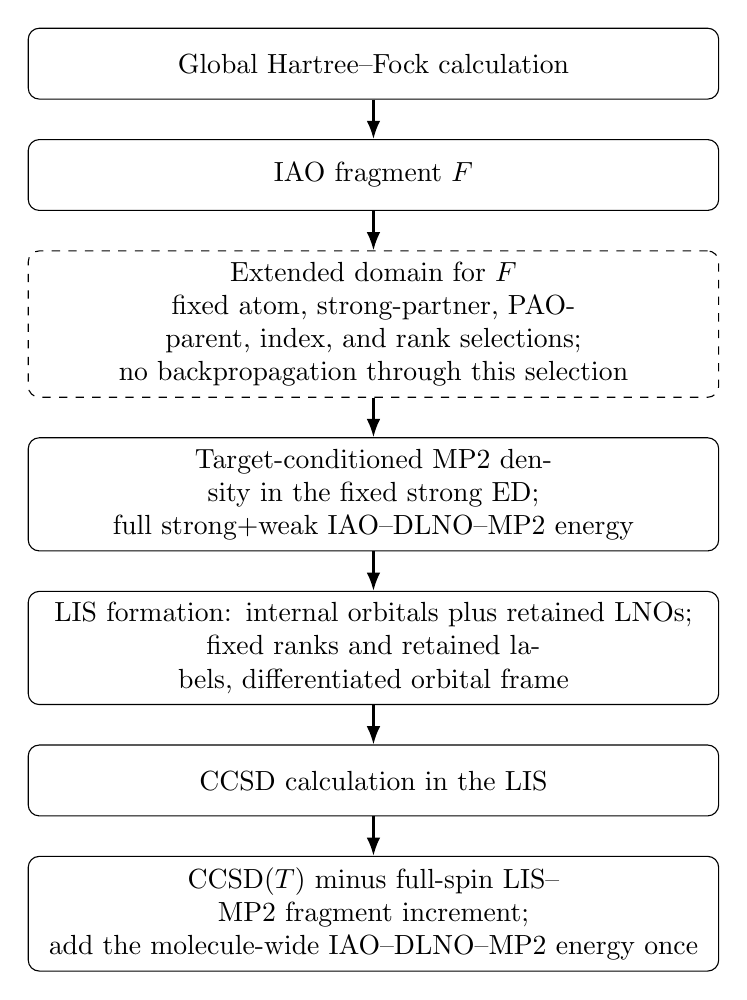
\begin{tikzpicture}[
      node distance=5mm,
      workflow/.style={
        draw,
        rounded corners,
        align=center,
        text width=0.70\textwidth,
        minimum height=9mm,
        inner sep=4pt
      },
      fixedworkflow/.style={workflow,dashed},
      flowarrow/.style={-{Latex},thick}
    ]
    \node[workflow] (scf) {Global Hartree--Fock calculation};
    \node[workflow,below=of scf] (iao) {IAO fragment $F$};
    \node[fixedworkflow,below=of iao] (ed)
      {Extended domain for $F$\\
       fixed atom, strong-partner, PAO-parent, index, and rank selections;\\
       no backpropagation through this selection};
    \node[workflow,below=of ed] (mp2)
      {Target-conditioned MP2 density in the fixed strong ED;\\
       full strong+weak IAO--DLNO--MP2 energy};
    \node[workflow,below=of mp2] (lis)
      {LIS formation: internal orbitals plus retained LNOs;\\
       fixed ranks and retained labels, differentiated orbital frame};
    \node[workflow,below=of lis] (ccsd) {CCSD calculation in the LIS};
    \node[workflow,below=of ccsd] (ccsdt)
      {CCSD$(T)$ minus full-spin LIS--MP2 fragment increment;\\
       add the molecule-wide IAO--DLNO--MP2 energy once};

    \draw[flowarrow] (scf) -- (iao);
    \draw[flowarrow] (iao) -- (ed);
    \draw[flowarrow] (ed) -- (mp2);
    \draw[flowarrow] (mp2) -- (lis);
    \draw[flowarrow] (lis) -- (ccsd);
    \draw[flowarrow] (ccsd) -- (ccsdt);
  \end{tikzpicture}
  \caption{Paper-level organization of the IAO-based local correlation
  calculation.  The dashed ED block performs only discrete selection and is
  held fixed during a nuclear derivative.  Numerical ED and LIS orbital
  frames retain their response.}
  \label{fig:iao-dlno-workflow}
\end{figure}

\subsection{Global Hartree--Fock calculation}

The inputs are the nuclear coordinates $\{\mathbf R_A\}$ and the AO and
auxiliary basis sets.  The outputs are
\begin{equation}
 E_{\mathrm{HF}},\quad S,\quad F,\quad C_o,\quad C_v,
 \quad \epsilon_o,\quad \epsilon_v,
 \label{eq:workflow-hf-output}
\end{equation}
together with the AO or density-fitted two-electron integrals.  The canonical
orbitals satisfy
\begin{equation}
 FC=SC\epsilon.
\end{equation}
This block is differentiated.  Its reverse response contains both explicit
nuclear derivatives of the AO integrals and the implicit SCF orbital response.
For the present local-MP2 derivative, the saved reverse map uses the standard
implicit response of the converged SCF fixed point.  The experimental
finite-iteration first-order replay is not used: a general local-orbital
correlation cotangent is nonstationary, so residual error in that replay can
be strongly amplified.  All gradients reported below use the standard
implicit SCF response.

\subsection{IAO fragment}

All IAOs assigned to the atoms of fragment $F$ are collected in the matrix
$A_F$.  In contrast to occupied-only localized orbitals, IAOs span the
occupied space and part of the valence-virtual space.  Their occupied and
virtual components must consequently be resolved separately
\cite{knizia2013,ye2024}:
\begin{equation}
 M_o^F=C_o^\dagger S A_F,
 \qquad
 M_v^F=C_v^\dagger S A_F.
 \label{eq:workflow-iao-projections}
\end{equation}
Separate singular-value decompositions define the internal occupied and
internal virtual spaces,
\begin{equation}
 O_F^{\mathrm{int}}=C_oI_o^F,
 \qquad
 V_F^{\mathrm{int}}=C_vI_v^F,
 \label{eq:workflow-internal-spaces}
\end{equation}
where $I_o^F$ and $I_v^F$ are the right-singular-vector matrices of
$B_o^F=A_F^\dagger SC_o$ and $B_v^F=A_F^\dagger SC_v$ in
Eq.~\eqref{eq:iao-lis-internal-anchors}.  Equivalently, they are the retained
left singular vectors of $M_o^F=(B_o^F)^\dagger$ and
$M_v^F=(B_v^F)^\dagger$.  The occupied fragment weight
\begin{equation}
 W_F=M_o^F(M_o^F)^\dagger
 \label{eq:workflow-fragment-weight}
\end{equation}
provides a positive-semidefinite resolution of the identity in the active
occupied space; for a complete orthonormal IAO partition,
$\sum_F W_F=I_o$.  All IAOs on the same atom or
functional group are treated together, making the construction invariant to
rotations among IAOs belonging to that fragment.  The coefficients and
subspaces in this block are differentiated, while their numerical ranks are
held fixed during one derivative evaluation.  The symmetric L\"owdin steps
retain their complete response through the divided-difference Fr\'echet
derivative of the inverse square root, including its degenerate limit.

\subsection{Fixed extended domain}

The ED construction takes the reference fragment spaces, PAOs, and
fragment-pair estimates as input.  The spatial selection is based on the
occupied component of the complete IAO block, not on separately normalized
IAOs.  Defining
\begin{equation}
 X_F=P_oA_F=C_oM_o^F,
 \qquad
 W_F=M_o^F(M_o^F)^\dagger,
 \label{eq:workflow-spatial-weight}
\end{equation}
$X_F$ is used to select atoms, whereas the generally non-idempotent $W_F$ is
retained for the additive energy partition.  The fraction of the occupied
fragment weight recoverable in the AO span of an atom set $D$ is
\begin{equation}
 \eta_F(D)=
 \frac{\operatorname{Tr}\!\left[
 X_F^\dagger S_{:D}S_{DD}^{-1}S_{D:}X_F
 \right]}
 {\operatorname{Tr}[X_F^\dagger SX_F]}.
 \label{eq:workflow-collective-bp}
\end{equation}
Atoms are added until three occupied-space completeness thresholds give a
compact BP list $\mathcal B_F^{\mathrm{occ}}$, a primary BP list
$\mathcal B_F^{\mathrm{prim}}$, and a tighter ED BP list
$\mathcal B_F^{\mathrm{ED}}$.  Because Eq.~\eqref{eq:workflow-collective-bp}
is a trace over the whole fragment block, the construction is invariant to a
unitary rotation among the IAOs assigned to $F$ and does not promote a
small-weight singular direction into an equally weighted occupied orbital.

The primary domain used for multipole pair screening is
\begin{equation}
 \mathcal P_F=
 \mathcal B_F^{\mathrm{prim}}\cup
 \bigcup_{A\in\mathcal B_F^{\mathrm{prim}}}
 \ \bigcup_{p\,\mathrm{centered\ on}\,A}
 \mathcal B_p^{\mathrm{PAO}},
 \label{eq:workflow-iao-primary}
\end{equation}
where $\mathcal B_p^{\mathrm{PAO}}$ is the BP atom list of PAO $p$.
Diagonalizing the occupied weight,
$W_Fu_{F\alpha}=w_{F\alpha}u_{F\alpha}$, gives normalized occupied modes
only for evaluating the inexpensive multipole estimate.  At the reference
geometry define
$\mathcal K_F^w=\{\alpha:w_{F\alpha}>\tau_{\mathrm{occ}}\}$.  The retained
labels and degenerate-block structure are fixed, while their values and
eigenspaces are rebuilt at the current geometry.  Within a nearly degenerate
block the occupied Fock matrix is diagonalized and the block is assigned its
mean weight, avoiding an arbitrary IAO gauge.  The retained weights remain in
the fragment-pair estimate,
\begin{equation}
 \widetilde E_{FG}^{(2)}=
 \sum_{\alpha\in\mathcal K_F^w}
 \sum_{\beta\in\mathcal K_G^w}
 w_{F\alpha}w_{G\beta}
 \widetilde E_{\alpha\beta}^{(2)}.
 \label{eq:workflow-weighted-pair-estimate}
\end{equation}
The strong-partner set is then
\begin{equation}
 \mathcal S_F=\{F\}\cup
 \left\{G:\left|\widetilde E_{FG}^{(2)}\right|>
 \tau_{\mathrm{pair}}\right\}
 \cup\mathcal S_F^{\mathrm{near/fail}}.
 \label{eq:workflow-strong-set}
\end{equation}
Geometrically near pairs, and pairs for which a stable multipole screening
space cannot be constructed, are forced into
$\mathcal S_F^{\mathrm{near/fail}}$.

Two unions with different roles are formed from the same strong set:
\begin{equation}
 \mathcal B_F^+=
 \bigcup_{G\in\mathcal S_F}\mathcal B_G^{\mathrm{occ}},
 \qquad
 \mathcal D_F=
 \bigcup_{G\in\mathcal S_F}\mathcal B_G^{\mathrm{ED}}.
 \label{eq:workflow-two-ed-lists}
\end{equation}
$\mathcal B_F^+$ selects the parent centers of candidate PAOs, while
$\mathcal D_F$ supplies the AO support of the numerical ED.  The local
auxiliary basis is generated on the atoms in $\mathcal D_F$; it is not an
independently selected atom list.  Thus the compact ED follows the improved
construction of Ref.~\cite{nagy2016}, rather than the older union of primary
domains.

The resulting discrete topology can be written as
\begin{equation}
 \mathcal T_F=
 \left\{
   \mathcal I_F,\mathcal S_F,\mathcal P_F,
   \mathcal B_F^+,\mathcal D_F,\mathcal K_F
 \right\},
 \label{eq:workflow-static-topology}
\end{equation}
where $\mathcal I_F$ identifies the IAOs belonging to $F$ and
$\mathcal K_F$ collects all threshold-selected labels and ranks.  These
include active occupied and virtual MO indices, the MO indices projected out
when forming PAOs, retained parent-AO/PAO columns, occupied-range indices, PAO
canonical-overlap and completeness indices, final metric indices, weak-mode
indices and degenerate blocks, and the strong/weak mask.  They are evaluated
at the reference geometry and held
fixed during the derivative.  We denote this fixed-branch convention by
\begin{equation}
 \left.\frac{d\mathcal T_F}{d\mathbf R_A}\right|_{\mathrm{fixed\ topology}}
 \equiv0,
 \qquad
 \overline{\mathcal T}_F=0.
 \label{eq:workflow-static-gradient}
\end{equation}
No numerical domain-orbital coefficients are included in $\mathcal T_F$.

\subsection{MP2 calculation in the fixed ED}

This block takes the current $S$, $F$, $C_o$, $C_v$, the IAO fragment spaces,
$W_F$, and the fixed topology $\mathcal T_F$.  It first reconstructs the
geometry-dependent orbitals on the selected atoms.  The strong-union occupied
weight is
\begin{equation}
 W_{\mathcal S_F}=\sum_{G\in\mathcal S_F}W_G,
 \qquad
 W_{\mathcal S_F}U_F
 =U_F\operatorname{diag}(\boldsymbol\omega_F).
 \label{eq:workflow-strong-weight}
\end{equation}
The eigenvectors whose reference eigenvalues pass the fixed occupied-weight
selection in $\mathcal K_F$ are projected into the AO span of
$\mathcal D_F$,
\begin{equation}
 \widetilde C_{o,F}=
 S_{\mathcal D_F\mathcal D_F}^{-1}S_{\mathcal D_F:}
 C_oU_F[:,\mathcal K_F^{o}].
 \label{eq:workflow-ed-occupied-projection}
\end{equation}
They are metric-orthonormalized to form the occupied ED space.  The virtual ED
space is constructed only from PAOs whose parent AOs are centered on
$\mathcal B_F^+$.  Raw PAOs are parent AOs projected into the active virtual
space; equivalently, frozen occupied, active occupied, and frozen virtual MOs
are projected out.  The reference construction records the surviving parent
columns, canonical PAO rank, local-overlap eigenvector indices, completeness
indices, and final metric indices.  At the current geometry all continuous
operations are replayed with those fixed index sets.  If $\overline P$ is the
current orthonormal parent-PAO span, its recoverable overlap on an atom set
$X$ is obtained from
\begin{equation}
 H_X=\overline P^\dagger
 S_{:X}S_{XX}^{-1}S_{X:}\overline P.
 \label{eq:workflow-pao-recoverable-overlap}
\end{equation}
For a strong ED, $X=\mathcal D_F$, the representation atoms are also
$\mathcal D_F$, and the final completeness threshold is
$\tau_{\mathrm{ED,PAO}}$.  For a weak multipole screen,
$X=\mathcal B_F^{\mathrm{prim}}$, the representation atoms are
$\mathcal P_F$, and the final completeness threshold is
$\tau_{\mathrm{BP,PAO}}$.  The retained candidates are projected into the
representation AO space and orthogonalized against its occupied span.  No
separate internal-valence virtual block is appended in the present
IAO--MP2 implementation.

More explicitly, let $C$ denote any projected occupied or PAO coefficient
block and let $\mathcal K$ be its fixed reference metric selection.  For a
truncated block, the current metric eigenvectors reconstruct the selected
span, which is then normalized by a differentiable Cholesky factorization,
\begin{equation}
 G=C^\dagger S_D C,\qquad
 Y=CV_G[:,\mathcal K],\qquad
 Y^\dagger S_DY=L_{\mathcal K}L_{\mathcal K}^\dagger,\qquad
 Q=YL_{\mathcal K}^{-\dagger}.
 \label{eq:workflow-fixed-metric-frame}
\end{equation}
If all columns are retained, $Y=C$ and no metric eigendecomposition is
required.  Thus only the retained labels and rank are static; the selected
subspace, metric, and Cholesky factor retain their complete nuclear response.
The occupied and virtual spaces are then semicanonicalized,
\begin{equation}
 F_{oo}^{\mathrm{ED}}U_o=U_o\epsilon_o^{\mathrm{ED}},
 \qquad
 F_{vv}^{\mathrm{ED}}U_v=U_v\epsilon_v^{\mathrm{ED}}.
 \label{eq:workflow-ed-semicanonical}
\end{equation}
The density-fitted integrals are transformed directly into the resulting
domain-sized spaces,
\begin{equation}
 (ia|jb)_F=\sum_{P\in\mathcal Q_F^{\mathrm{aux}}}
 L_{Pia}^{F}L_{Pjb}^{F},\qquad
 i\in O_F^{\mathrm{ED}},\quad
 a\in V_F^{\mathrm{ED}}.
 \label{eq:workflow-domain-lov}
\end{equation}
Here $P$ labels an auxiliary function in the local auxiliary basis
$\mathcal Q_F^{\mathrm{aux}}$ generated on $\mathcal D_F$, rather than an
atom.  In the integral-direct implementation the raw three-center integrals
are transformed to the occupied--virtual representation before storage, so a
full AO-pair density-fitting tensor and full four-index ERIs are not formed.
For the reverse transformation, let $J=KK^\dagger$ be the local auxiliary
metric factorization, let $Y_{Pia}$ be the raw transformed three-center
tensor, and write
\begin{equation}
 L_{Pia}=\left(K^{-1}Y\right)_{Pia},\qquad
 Z_{Pia}=\left(K^{-\dagger}\overline L\right)_{Pia},\qquad
 D_{P\mu\nu}=\sum_{ia}C^o_{\mu i}Z_{Pia}C^v_{\nu a}.
 \label{eq:workflow-direct-ri-reverse}
\end{equation}
The AO-center derivative then contracts the symmetrized density
$D_{P\mu\nu}+D_{P\nu\mu}$ with the derivative three-center integrals once.
The contraction order is selected so that the AO-square intermediate carries
$\min(n_o,n_v)$: for $n_o\leq n_v$ the virtual index is contracted first,
$T_{Pi\nu}=\sum_a Z_{Pia}C^v_{\nu a}$, followed by
$D_{P\mu\nu}=\sum_i C^o_{\mu i}T_{Pi\nu}$; the opposite order is used when
$n_v<n_o$.  This changes the leading AO-center work from two derivative
integral transforms, $O(3Pn_{\mathrm{AO}}^2(n_o+n_v))$, to
$O(Pn_{\mathrm{AO}}n_on_v+Pn_{\mathrm{AO}}^2\min(n_o,n_v))$ plus the final
derivative contraction.  Only $L_{Pia}$ is retained: neither a packed local
AO-pair CDERI nor a full $ovov$ tensor is allocated.
The present reverse implementation requires the local auxiliary metric to be
sufficiently positive definite for Cholesky factorization; the forward-only
eigenvalue fallback for a linearly dependent auxiliary basis is deliberately
rejected in a nuclear derivative until its response is implemented.
The first-order amplitudes are
\begin{equation}
 t_{ij}^{ab,F}=
 \frac{(ia|jb)_F}
 {\epsilon_i^F+\epsilon_j^F-\epsilon_a^F-\epsilon_b^F}.
 \label{eq:workflow-domain-mp2-amplitude}
\end{equation}
Writing $A_{\mathcal S_F}$ for the concatenated IAO blocks of the strong
partners, their weights represented in the semicanonical occupied ED are
\begin{align}
 Z_F&=A_F^\dagger S_{:\mathcal D_F}C_{o,F}^{\mathrm{ED}}, &
 W_F^{\mathrm{ED}}&=Z_F^\dagger Z_F,\\
 Z_{\mathcal S_F}&=A_{\mathcal S_F}^\dagger
 S_{:\mathcal D_F}C_{o,F}^{\mathrm{ED}}, &
 W_{\mathcal S_F}^{\mathrm{ED}}
 &=Z_{\mathcal S_F}^\dagger Z_{\mathcal S_F}.
 \label{eq:workflow-ed-fragment-weights}
\end{align}
The strong contribution places the target-fragment weight on one occupied
line and the strong-union weight on the other,
\begin{equation}
 E_F^{\mathrm{strong}}=
 \sum_{pqrsab}
 (W_F^{\mathrm{ED}})_{pq}
 (W_{\mathcal S_F}^{\mathrm{ED}})_{rs}
 t_{pr}^{ab,F}
 \left[2(qa|sb)_F-(qb|sa)_F\right].
 \label{eq:workflow-weighted-strong-energy}
\end{equation}
Pairs excluded from $\mathcal S_F$ are not discarded.  Their multipole MP2
increments are added with symmetric bookkeeping,
\begin{equation}
 E_F^{\mathrm{local}(2)}=
 E_F^{\mathrm{strong}}+
 \frac12\sum_{G\notin\mathcal S_F}
 \widetilde E_{FG}^{(2)},
 \qquad
 E_{\mathrm{IAO\mbox{-}LMP2}}=\sum_F E_F^{\mathrm{local}(2)}.
 \label{eq:workflow-local-mp2-energy}
\end{equation}
The factor $1/2$ counts each unordered weak fragment pair once.  All
continuous transformations in this block are differentiated: the IAOs and
PAOs, $W_F$, projected and semicanonical orbitals, local RI factors,
denominators, strong-pair energy, and all multipole moments and pair energies.
Thus the ED topology is fixed, but every numerical quantity represented on it
retains its nuclear response.

For the total energy, the equivalent upper-triangular implementation is
\begin{equation}
 E_{\mathrm{IAO\mbox{-}LMP2}}
 =\sum_F E_F^{\mathrm{strong}}
 +\sum_{F<G,\,FG\ \mathrm{weak}}\widetilde E_{FG}^{(2)}.
 \label{eq:workflow-local-mp2-upper-triangle}
\end{equation}
Each strong ED and each unordered weak pair is differentiated with its own
reverse map.  Its cotangent is accumulated immediately and its tape is
released before the next scalar contribution.  The peak reverse tape is
therefore set by one strong ED or one weak pair, rather than by all weak
partners of a fragment.  The common IAO/PAO data are rebuilt once under a
saved reverse map, closed once after all contributions have been accumulated,
and then passed through a single implicit SCF response.

The weak multipole path also batches all retained occupied modes of an
endpoint.  With mode $\phi_\alpha$, shared PAO $\chi_a$, center
$R_{\alpha x}=\langle\phi_\alpha|r_x|\phi_\alpha\rangle$, and
$\sigma_{\alpha a}=\langle\chi_a|\phi_\alpha\rangle$, the origin-zero
transition moments $d^0$, $M^{(2),0}$, and $M^{(3),0}$ are formed from one
set of AO overlap, dipole, quadrupole, and octupole operators per endpoint.
Translation is then performed in the smaller MO transition space,
\begin{align}
 M^{(2)}_{xy}
 &=M^{(2),0}_{xy}-R_xd^0_y-R_yd^0_x+R_xR_y\sigma,\\
 M^{(3)}_{xyz}
 &=M^{(3),0}_{xyz}-R_xM^{(2),0}_{yz}-R_yM^{(2),0}_{xz}
   -R_zM^{(2),0}_{xy}\notag\\
 &\quad+R_xR_yd^0_z+R_xR_zd^0_y+R_yR_zd^0_x-R_xR_yR_z\sigma.
 \label{eq:workflow-batched-multipole-translation}
\end{align}
The translated tensors are subsequently detraced.  This replaces replicated
AO moment operators for every occupied mode by one AO operator set plus a
batch of much smaller MO-space tensors.  Modes with heterogeneous atom lists
or rectangular dimensions are partitioned into compatible batches; a
singleton group still uses the same batched implementation.

The accumulated local correlation cotangent is finally closed through the
standard fixed-point implicit SCF response described above.  This separates
the static selection boundary from the continuous AO-integral, orbital, IAO,
PAO, RI, denominator, and multipole responses.

The local-MP2 gradient implementation returns the energy in
Eq.~\eqref{eq:workflow-local-mp2-energy} and its cotangents.  The implemented
LIS path reuses each strong-ED amplitude to construct the target-conditioned
occupied and virtual selection densities in
Eqs.~\eqref{eq:iao-lis-density-oo} and
\eqref{eq:iao-lis-density-vv}.  Their ranks and retained labels are fixed at
the reference geometry, while their floating-point construction remains in
the differentiated program.  These are unrelaxed LNO-selection densities,
not the relaxed density entering a conventional analytic MP2 gradient.  The
large-system benchmark in Sec.~\ref{sec:pair-cutoff-results} deliberately
isolates the local-MP2 energy and gradient branch; the complete LIS and CC
driver is validated separately in Sec.~\ref{sec:small-cc-validation}.

\subsubsection{Reverse-mode AD and propagation through the mean field}
\label{sec:iao-mp2-mf-cotangent}

The present IAO--DLNO--MP2 nuclear derivative is not a separately
hand-derived MP2 Lagrangian gradient.  The fixed-topology scalar energy is
written as a differentiable program and its vector--Jacobian products (VJPs)
are evaluated with reverse-mode automatic differentiation.  The strong-ED
MP2 contractions, amplitudes and denominators, IAO and PAO reconstruction,
fragment weights, local orbital projections, semicanonicalizations, and weak
multipole energies are differentiated directly.

The implementation is nevertheless hybrid at the level of numerical
primitives.  Operations whose naive AD trace would be prohibitively large,
or which call external integral code, provide custom analytic derivative
rules.  In particular, the integral-direct RI transformation uses
Eq.~\eqref{eq:workflow-direct-ri-reverse} to return coordinate,
auxiliary-metric, and MO-coefficient cotangents without storing a full
AO-pair CDERI.  Cartesian AO moments, the symmetric L\"owdin matrix function,
and selected integral transformations also have custom JVPs or VJPs.  The
converged SCF map is closed by an implicit fixed-point pullback.  These are
hand-written primitive derivatives, but there is no hand-assembled local-MP2
relaxed density, two-particle density, or local-MP2 Z-vector formula.

Let $\mathcal M=M(\mathbf R)$ denote the differentiable mean-field state and
let $\mathcal T$ denote the fixed topology.  The state $\mathcal M$ includes
the molecule and DF objects, the canonical coefficients and orbital energies,
and the HF energy.  The reverse calculation can be factored as
\begin{equation}
 q=G(\mathcal M;\mathcal T),\qquad
 y_k=H_k(q;\mathcal T),\qquad
 E_{\mathrm{corr}}=\sum_k e_k(\mathcal M,y_k;\mathcal T),
 \label{eq:mf-cotangent-factorization}
\end{equation}
where $q$ contains the common overlap, Fock, IAO, PAO, and fragment-weight
data.  The object $y_k$ is either one numerical strong-ED frame or the two
endpoint screens of one unordered weak pair.  The index $k$ therefore runs
over every strong row and every unordered weak pair exactly once.

With a unit cotangent on each scalar term, reverse mode gives
\begin{align}
 \left(\overline{\mathcal M}^{\,\mathrm{dir}}_k,\bar y_k\right)
   &=\operatorname{VJP}[e_k](1),\notag\\
 \bar q
   &=\sum_k\operatorname{VJP}[H_k](\bar y_k),\notag\\
 \overline{\mathcal M}_{\mathrm{corr}}
   &=\sum_k\overline{\mathcal M}^{\,\mathrm{dir}}_k
     +\operatorname{VJP}[G](\bar q).
 \label{eq:mf-cotangent-assembly}
\end{align}
The direct term contains, for example, the response of the local three-center
integrals or multipole operators evaluated from $\mathcal M$.  The second
term propagates the orbital-frame cotangents through the shared IAO/PAO
construction.  These are independent occurrences of the same mean-field
state, so their cotangents are added rather than identified as duplicate
response.  Each scalar term is pulled back and its tape is released before
the next term; peak reverse storage is therefore set by one strong ED or one
weak pair.

The object $\overline{\mathcal M}_{\mathrm{corr}}$ is the
\texttt{mf\_bar} returned by the reusable correlation-gradient routine.  It
is a structured PyTree cotangent defined by
\begin{equation}
 dE_{\mathrm{corr}}
 =\left\langle
   \overline{\mathcal M}_{\mathrm{corr}},d\mathcal M
  \right\rangle_{\mathrm{tree}}.
 \label{eq:mf-bar-definition}
\end{equation}
It can contain cotangents of canonical MO coefficients, orbital energies,
molecular coordinates, auxiliary-molecule data, and the DF state.  It is not
itself a one-particle density matrix and need not be invariant under a change
of orbital coordinates.  Correlation cotangents from IAO--DLNO--MP2,
CCSD(T) fragments, and the LIS-MP2 subtraction can nevertheless be added at
this boundary, provided that all are expressed in the same mean-field gauge.
Including the HF reference additionally seeds the \texttt{e\_tot} leaf with
a unit cotangent.

To expose the final nuclear response, write the converged SCF equations as
\begin{equation}
 D^\star=\Phi(D^\star,\mathbf R),\qquad
 \mathcal M=\mathcal H(D^\star,\mathbf R).
 \label{eq:scf-fixed-point-map}
\end{equation}
For an incoming mean-field cotangent $\overline{\mathcal M}$, the implicit
reverse map first forms
\begin{equation}
 \bar D=\mathcal H_D^\dagger\overline{\mathcal M},\qquad
 (I-\Phi_D^\dagger)z=\bar D,
 \label{eq:scf-adjoint}
\end{equation}
and then returns
\begin{equation}
 \bar{\mathbf R}
 =\mathcal H_{\mathbf R}^\dagger\overline{\mathcal M}
  +\Phi_{\mathbf R}^\dagger z.
 \label{eq:scf-nuclear-cotangent}
\end{equation}
For an RHF reference this transposed fixed-point solve is the AD analogue of
the usual CPHF or Z-vector response.  Incoming MO-coefficient and
orbital-energy cotangents are first propagated through the final Fock
diagonalization and Fock construction, thereby generating the density-matrix
source $\bar D$ and explicit AO-integral terms.  Thus the public intermediate
is a gauge-coordinate-dependent mean-field cotangent, whereas the deepest
SCF response equation is based on the full AO-density fixed point.  Neither
$\bar D$ nor $z$ should be identified directly with a conventional relaxed
one-particle density.  One implicit solve is applied after all post-SCF
cotangents have been accumulated; that solve generally contains many
applications of the transposed SCF Jacobian.

\paragraph{Difference from a conventional occupied--virtual CPHF solve.}
For closed-shell RHF, the fixed-point map used here is the converged
Roothaan map
\begin{equation}
 F[D;\mathbf R]=h(\mathbf R)+\mathcal G_{\mathbf R}[D],
 \qquad
 \Phi(D,\mathbf R)=2C_o(F[D;\mathbf R],S[\mathbf R])C_o^\dagger,
 \qquad C^\dagger SC=I.
 \label{eq:rhf-roothaan-map}
\end{equation}
DIIS and damping may be used to reach $D^\star$, but their iteration history
is not differentiated.  For comparison, at fixed AO overlap conventional
RHF CPHF parameterizes the first-order density by occupied--virtual orbital
rotations $U_{ai}$.  If $C_o$ and $C_v$ denote the converged occupied and
virtual canonical orbitals, its response equation can be written
schematically as
\begin{align}
 D^{(1)}[U]
 &=2\left(C_vUC_o^\dagger+C_oU^\dagger C_v^\dagger\right),\notag\\
 \mathcal A_{ov}[U]
 &=(\epsilon_a-\epsilon_i)U_{ai}
   +\left[C_v^\dagger\mathcal G_D[D^{(1)}[U]]C_o\right]_{ai}
   =R_{ai},
 \label{eq:conventional-ov-cphf}
\end{align}
where $\mathcal G_D$ is the RHF Coulomb--exchange response, including the
occupation factors.  In an analytic gradient the transposed equation
$\mathcal A_{ov}^\dagger Z=L_{ov}$ is normally solved for an orbital-gradient
source $L_{ov}$.  The unknown therefore contains only $n_vn_o$ elements,
and the diagonal orbital gaps supply a natural preconditioner.  Relaxed and
energy-weighted AO densities are assembled after this solve.

Equations~\eqref{eq:scf-adjoint} and
\eqref{eq:scf-nuclear-cotangent} use different coordinates for the same
self-consistent response.  The implemented multiplier $z$ is an AO-density
matrix and GMRES applies the transpose of the complete converged density map,
\begin{equation}
 z\longmapsto\Phi_D^\dagger z,
 \qquad
 (I-\Phi_D^\dagger)z=\mathcal H_D^\dagger
                         \overline{\mathcal M}.
 \label{eq:ao-density-scf-adjoint}
\end{equation}
It is consequently not numerically identical to the conventional
occupied--virtual $Z_{ai}$ vector.  On the regular RHF tangent space the two
linear systems encode the same coupled orbital relaxation, but the AO
fixed-point form also carries redundant density coordinates and uses no
separately supplied GMRES preconditioner.  The inverse gaps already enter
$\Phi_D$ through differentiation of the Roothaan diagonalization, so the
occupied--virtual restriction is a gap-left-preconditioned form of CPHF;
it is nevertheless represented and iterated in the full AO space.  For the
C16/cc-pVTZ example the respective dimensions are $956^2=913936$ AO-density
entries and $65\times891=57915$ occupied--virtual entries.

The broader source in Eq.~\eqref{eq:ao-density-scf-adjoint} is important for
the present local functional.  A conventional MP2 or CC Lagrangian first
reduces its response to relaxed, gauge-invariant AO density intermediates, so
only its assembled occupied--virtual orbital-gradient source crosses the CPHF
interface.  Here the incoming object is instead the structured cotangent
$\overline{\mathcal M}$.  It contains the full $\bar C$ and
$\bar\epsilon$ generated by IAO and PAO reconstruction, ED and LIS
projections, semicanonicalizations, local denominators, and fragment weights.
The components of $\bar C$ within occupied or virtual coordinate blocks
cannot simply be discarded: before the self-consistent occupied--virtual
response is isolated, the full generalized-eigensystem VJP must convert them
into explicit Fock and overlap cotangents in the same primal gauge.  The
AO-density fixed-point pullback performs this complete chain rule
automatically.

More explicitly, define
\begin{equation}
 U=C^\dagger S\,dC,\qquad
 S_C^{(1)}=C^\dagger(dS)C,\qquad
 X=C^\dagger(dF)C-S_C^{(1)}\epsilon.
 \label{eq:generalized-eigen-response-definitions}
\end{equation}
For a nondegenerate generalized eigensystem in the selected canonical gauge,
\begin{equation}
 d\epsilon_p=X_{pp},\qquad
 U_{pq}=\frac{X_{pq}}{\epsilon_q-\epsilon_p}\;(p\ne q),\qquad
 U_{pp}=-\frac12(S_C^{(1)})_{pp},\qquad dC=CU.
 \label{eq:generalized-eigen-response}
\end{equation}
The reverse rule is the transpose of this entire map, defined by
\begin{equation}
 \langle\bar C,dC\rangle_{\mathbb R}
 +\langle\bar\epsilon,d\epsilon\rangle_{\mathbb R}
 =\langle\bar F,dF\rangle_{\mathbb R}
 +\langle\bar S,dS\rangle_{\mathbb R}.
 \label{eq:generalized-eigen-transpose}
\end{equation}
Thus orbital-energy, overlap-normalization, and same-space orbital-coordinate
terms are converted before the coupled response is reduced to its physical
occupied--virtual tangent.  The implementation sets inverse gaps to zero
inside its degeneracy threshold; a raw gauge-coordinate objective is not
differentiable at an unresolved exact degeneracy.

A future exact occupied--virtual implementation can be equivalent and more
efficient, but it must first transpose the full map
$(F,S)\mapsto(C,\epsilon)$, retain its explicit $\bar F$ and $\bar S$
terms, construct only the density-coupled $L_{ov}$ source, solve the
transposed CPHF equation, and finally add the explicit terms.  Applying a
standard MP2 CPHF routine directly to a projection of $\bar C$ would lose
the same-space and gauge-coordinate contributions.  This is also why all MPI
cotangents must be accumulated in one root-selected orbital gauge before the
SCF response is closed.

\paragraph{Density-only DF--JK transpose in the implemented adjoint.}
The fixed-point representation does not require nuclear or density-fitting
factor cotangents during a GMRES matrix--vector product.  In that operation
the geometry, auxiliary basis, and fitted three-center factors are closed-over
constants; only the transpose action with respect to $D$ is used.  If the
real symmetric fitted factors are denoted by AO matrices $B_P$, then the
required Coulomb and exchange contributions are
\begin{align}
 \bar D_J
 &\mathrel{+}=\sum_P B_P\,\langle B_P,\bar J\rangle_{\mathbb R},\notag\\
 \bar D_K
 &\mathrel{+}=\sum_P B_P\bar K B_P.
 \label{eq:dfjk-density-only-transpose}
\end{align}
The signs and RHF factors enter through the upstream cotangents $\bar J$ and
$\bar K$.  The Coulomb transpose uses the existing streamed packed-BLAS
contractions, while a new native density-only kernel evaluates the exchange
transpose.  Both omit every term that would contribute only to $\bar B_P$.

Previously the generic DF--JK VJP also constructed $\bar B_P$ during every
GMRES application, even though JAX discarded it.  For C16/cc-pVTZ this meant
an $n_{\rm aux}\times n_{\rm pair}=2316\times457446$ float64 cotangent,
or 7.893~GiB logically, followed by repeated three-center, auxiliary-metric,
and Cholesky pullbacks.  The implicit-differentiation driver now marks only
the solution-Jacobian scope.  Within that scope the DF--JK rule returns
$(0,\bar D)$ for the DF object and density inputs, respectively: it allocates
neither a full in-memory $\bar B$, an out-of-core $\bar B$ file, nor the
associated nuclear derivative.  After the linear solve, the unchanged
external-argument VJPs evaluate all required molecular, three-center,
metric, and Cholesky derivatives.
The persisted primal out-of-core CDERI is still streamed.  The Krylov-phase
reverse workspace is one auxiliary block plus
$O(n_{\rm thread}n_{\rm AO}^2)$ exchange work arrays, rather than an
$O(n_{\rm aux}n_{\rm pair})$ factor cotangent.

On a deterministic out-of-core H$_2$O/cc-pVQZ test with a general
MO-coefficient and orbital-energy cotangent, the value and nuclear gradient
were unchanged bit for bit.  Ten GMRES applications became density-only and
the number of complete DF coordinate VJPs fell from 13 to 3.  Across three
fresh-process measurements, the median saved-SCF-pullback time decreased
from 3.5575 to 1.7889~s, while median accumulated coordinate-VJP time
decreased from 2.1158 to 0.6009~s.  This test demonstrates removal of the
redundant work; it is not an extrapolated C16 timing.  The remaining
post-solve coordinate VJPs are genuine occurrences in the present output and
external-argument graph.

The optimized response remains the converged AO-density fixed-point adjoint,
not the experimental ``first-order custom'' SCF backend.  That older backend
differentiates a finite replay of the SCF iteration history rather than
solving CPHF, and its residual dependence is unsuitable for the general
nonstationary local-orbital cotangent.  Tracer and higher-order cases retain
the generic derivative fallback.  Replacing the AO-density GMRES with the
carefully assembled occupied--virtual adjoint described above is a separate
optimization.

\paragraph{Relation to a conventional PySCF MP2 gradient.}
The conventional four-index PySCF MP2 gradient \cite{sun2018} organizes the same chain rule
as a hand-written stationary Lagrangian.  MP2 amplitudes generate unrelaxed
one-particle blocks and a partially AO-transformed two-particle density; an
orbital-gradient source is closed by one CPHF solve to form a relaxed density
and energy-weighted density.  The final derivative has the schematic AO form
\begin{equation}
 dE=\operatorname{Tr}[D_{\mathrm{rel}}^{(1)}\,dh]
   +\frac12\operatorname{Tr}[\Gamma_{\mathrm{rel}}^{(2)}\,dg]
   -\operatorname{Tr}[X\,dS]+dE_{\mathrm{nuc}},
 \label{eq:conventional-mp2-gradient}
\end{equation}
with the two-electron term reorganized into three-center and auxiliary-metric
contractions in a DF formulation.  Current PySCF DF-MP2 provides the relaxed
density machinery but not a complete nuclear-gradient driver; the explicit
nuclear-gradient implementation is the conventional four-index MP2 route.

The density-matrix interpretation is therefore directionally correct,
but a qualification is important.  PySCF does not pass only the HF density
matrix ``to MP2.''  Its MP2 energy still uses canonical orbitals, orbital
energies, and amplitudes, and the gradient requires a relaxed one-particle
density, a two-particle or DF three-center density, an energy-weighted density,
and the CPHF response.  Individual MO intermediates are gauge covariant; only
after they are consistently transformed and contracted are the final AO
Lagrangian objects independent of the allowed canonical-orbital gauge.

The present implementation instead retains orbital-coordinate cotangents
until they are closed through the common orbital and SCF pullbacks.  This
avoids deriving a separate enlarged Lagrangian for every IAO, PAO,
fragment-weight, projected-ED, local-RI, weighted strong-pair, and weak
multipole operation.  A canonical MP2 relaxed density alone could not encode
these additional dependencies.  Away from topology changes and singular
eigenspace choices, the AD and Lagrangian formulations are two organizations
of the same chain rule and yield the same nuclear derivative.  In the
all-strong full-domain limit, the implementation is tested against canonical
DF-MP2 energies and nuclear gradients.

\paragraph{MPI gauge consistency.}
Although the scalar energy is invariant under an allowed orbital rotation,
its coordinate cotangent transforms with that rotation.  For a fixed unitary
$U$,
\begin{equation}
 C'=CU,\qquad \bar C'=\bar C U.
 \label{eq:orbital-cotangent-gauge}
\end{equation}
Here ``allowed'' includes signs, consistent permutations, and rotations within
a truly degenerate occupied or virtual subspace.  An arbitrary rotation among
nondegenerate canonical orbitals is not a gauge transformation of the
diagonal-denominator canonical MP2 expression.
Coefficient cotangents produced in independently selected sign conventions
or degenerate-subspace gauges therefore cannot be added component by
component: their components refer to different coordinate frames.

In the present MPI implementation of the IAO local-MP2 energy and gradient,
rank zero performs the SCF calculation, constructs the common IAO/PAO state,
and constructs the numerical strong-ED or weak-pair endpoint frames.  The
exact canonical state and root-gauge frames are distributed in bounded
batches.  Workers differentiate only
$e_k(\mathcal M,y_k)$ and return
$\overline{\mathcal M}^{\mathrm{dir}}_k$ and $\bar y_k$.  Rank zero
deterministically replays $H_k$, checks that the numerical primal frame is
unchanged, accumulates $\bar q$, applies the shared pullback $G^\dagger$, and
finally invokes the single SCF pullback.  No worker independently
diagonalizes an orbital frame whose cotangent is later applied to a
differently gauged primal.  A future AO-density/Lagrangian response interface
could remove this MPI gauge contract, but the present raw mean-field
cotangent interface is correct only with the shared root gauge.  Multi-rank
IAO--DLNO--CCSD(T) is not implemented at present and is deliberately
rejected.  A future distributed CCSD(T) driver must extend the same root-gauge
contract to every LIS, CC-amplitude, and triples cotangent before any
cross-rank sum is performed.

\subsection{Local interacting subspace formation}

The raw IAO block is resolved into the internal occupied and virtual anchors
of Eq.~\eqref{eq:iao-lis-internal-anchors}.  Singular directions that pass
the internal-rank screen are retained without subsequent density truncation.
The strong-ED densities are mapped separately into the complete
active HF occupied and virtual manifolds by
Eq.~\eqref{eq:iao-lis-global-density}, projected into the external
complements, and diagonalized,
\begin{equation}
 D_{oo}^{F,\mathrm{ext}}X_o=X_on_o,
 \qquad
 D_{vv}^{F,\mathrm{ext}}X_v=X_vn_v.
 \label{eq:workflow-lno-eigenproblem}
\end{equation}
External LNOs with significant occupation numbers are combined with the
internal spaces to form
\begin{align}
 O_F^{\mathrm{LIS}}
   &=O_F^{\mathrm{int}}\oplus O_F^{\mathrm{LNO}},\\
 V_F^{\mathrm{LIS}}
   &=V_F^{\mathrm{int}}\oplus V_F^{\mathrm{LNO}}.
 \label{eq:workflow-lis-spaces}
\end{align}
The retained/discarded occupation-number mask is held fixed for a derivative,
but the retained LNO subspaces and their separate occupied and virtual
semicanonicalizations are differentiated.  The complementary active
directions are included in the complete MO layout and frozen.  The molecular
Hamiltonian is transformed into the resulting LIS, and the conventional
full-spin MP2 fragment energy $E_{\mathrm{MP2},F}^{\mathrm{LIS}}$ is evaluated
in exactly the same space for the subtraction in
Eq.~\eqref{eq:iao-lmp2-cc-correction}.

\subsection{CCSD calculation in the LIS}

Let $i,j,p,q$ and $a,b$ label the occupied and virtual orbitals of the LIS for
fragment $F$.  The right-hand CCSD amplitudes $T_F=T_{1,F}+T_{2,F}$ obey the
ordinary, unweighted impurity equations
\begin{equation}
 R_\mu^F(t_F;x_F)=
 \langle\mu|e^{-T_F}H_F(x_F)e^{T_F}|0\rangle=0,
 \label{eq:lis-cc-residual}
\end{equation}
where $x_F$ denotes the LIS Hamiltonian and orbital data.  The IAO partition
enters the scalar energy, rather than the residual equations.  In particular,
\begin{equation}
 P_{Ii}^F=\langle A_{FI}|i_F\rangle,
 \qquad W^F=(P^F)^\dagger P^F,
 \label{eq:lis-fragment-projector}
\end{equation}
and the implemented closed-shell fragment energy can be written, for real
orbitals, as
\begin{align}
 E_{\mathrm{CCSD},F}
 &=\sum_{pq}W_{pq}^F\Bigg[
  2\sum_a t_p^a f_{qa}
  +\sum_{jab}\tau_{pj}^{ab}
   \left\{2(qa|jb)-(qb|ja)\right\}\Bigg],
 \notag\\
 \tau_{ij}^{ab}&=t_{ij}^{ab}+t_i^at_j^b.
 \label{eq:lis-weighted-cc-energy}
\end{align}
Numerically, the raw IAO block $A_F$ is passed to the impurity solver and its
overlap with the active occupied LIS produces $P^F$; its virtual component
instead enters through the rank-screened internal virtual anchor.  The same
occupied projector defines $E_{\mathrm{MP2},F}^{\mathrm{LIS}}$, with the
separate first-order doubles amplitudes in place of $\tau$.  The MP2
subtraction is consequently independent of the converged CCSD amplitudes.

\subsection{Perturbative triples and corrected molecular energy}

The perturbative triples contribution is evaluated using the LIS amplitudes,
integrals, orbital energies, and the same occupied fragment weight,
\begin{equation}
 E_{(T),F}=\mathcal E_{(T)}\!\left[
 W^F,t_{1,F},t_{2,F},\epsilon_F,f_{vo,F},
 v_{ovoo,F},v_{ovov,F},v_{ovvv,F}\right].
 \label{eq:lis-weighted-triples-functional}
\end{equation}
The CC improvement over MP2 in fragment $F$ is
\begin{equation}
 \Delta E_F^{\mathrm{CC}}
 =E_{\mathrm{CCSD}}^F+E_{(T)}^F
  -E_{\mathrm{MP2},F}^{\mathrm{LIS}},
 \label{eq:workflow-final-fragment-energy}
\end{equation}
and the complete molecule-wide local MP2 energy is then added once,
\begin{equation}
 E=E_{\mathrm{HF}}+\sum_F\Delta E_F^{\mathrm{CC}}
   +E_{\mathrm{IAO\mbox{-}LMP2}}^{\mathrm{strong+weak}}.
 \label{eq:workflow-total-energy}
\end{equation}
This is the same identity as Eq.~\eqref{eq:iao-lmp2-cc-correction}.  In
particular, each unordered weak pair occurs only once in the final scalar.  A
unit cotangent on the total energy therefore gives
\begin{equation}
 \overline E_{\mathrm{CCSD}}^F=1,
 \quad
 \overline E_{(T)}^F=1,
 \quad
 \overline E_{\mathrm{MP2,LIS}}^F=-1,
 \qquad
 \overline E_{\mathrm{IAO\mbox{-}LMP2}}=1.
 \label{eq:workflow-reverse-seeds}
\end{equation}
The last seed is decomposed internally into unit seeds on every strong ED row
and every unordered weak pair, followed by one closure of the common IAO
pullback.
At the paper level these branches fan into one common mean-field cotangent,
\begin{equation}
 \overline{\mathcal M}_{\mathrm{tot}}
 =\overline{\mathcal M}_{\mathrm{HF}}
  +\overline{\mathcal M}_{\mathrm{IAO\mbox{-}LMP2}}
  +\sum_F\left(
    \overline{\mathcal M}_{\mathrm{CCSD(T)},F}
    -\overline{\mathcal M}_{\mathrm{MP2,LIS},F}
  \right)
 \xrightarrow{\operatorname{VJP}[M]}
 \nabla_{\mathbf R}E,
 \label{eq:workflow-reverse-chain}
\end{equation}
where the shared IAO/local-orbital pullbacks are closed before the final arrow.
The ED-selection block of Eq.~\eqref{eq:workflow-static-topology} is bypassed
entirely.  The individual post-SCF branches are therefore differentiated in
parallel at the level of the chain rule rather than serially through one
another.

\subsection{CCSD(T) nuclear derivative: Lagrangian and fixed-point forms}
\label{sec:iao-dlno-cc-gradient}

For a real scalar $E$, define the cotangent of an array $y$ by the real
Frobenius pairing
\begin{equation}
 dE=\langle\bar y,dy\rangle_{\mathbb R},
 \qquad
 \langle a,b\rangle_{\mathbb R}
 =\operatorname{Re}\sum_\alpha a_\alpha^*b_\alpha
 =\operatorname{Re}\!\left[\operatorname{vec}(a)^\dagger
                              \operatorname{vec}(b)\right].
 \label{eq:cc-real-cotangent}
\end{equation}
The following equations make explicit which response equations are solved and
how they differ in representation from a conventional hand-written
CCSD(T) gradient.

\subsubsection{Conventional CC and CCSD(T) Lagrangians}

First define the part of the fragment scalar that depends on the converged
CCSD amplitudes,
\begin{equation}
 \phi_F(t_F,x_F)=E_{\mathrm{CCSD},F}(t_F,x_F)
                  +E_{(T),F}(t_F,x_F),
 \qquad
 b_F=\left(\frac{\partial\phi_F}{\partial t_F}\right)^\dagger .
 \label{eq:cc-fragment-objective}
\end{equation}
The LIS--MP2 subtraction uses separate first-order amplitudes and is not
included in $b_F$.  A conventional analytic derivation augments the scalar
with the projected residuals in Eq.~\eqref{eq:lis-cc-residual},
\begin{equation}
 \mathcal L_F^{\mathrm{CC}}
 =\phi_F(t_F,x_F)
  +\langle\Lambda_F,R_F(t_F,x_F)\rangle_{\mathbb R}.
 \label{eq:conventional-cc-lagrangian}
\end{equation}
Stationarity with respect to the right amplitudes gives the left-amplitude
or Lambda equations
\begin{equation}
 J_{R,F}^\dagger\Lambda_F=-b_F,
 \qquad
 J_{R,F}=\frac{\partial R_F}{\partial t_F},
 \label{eq:conventional-cc-adjoint}
\end{equation}
and the cotangent of any external fragment quantity is
\begin{equation}
 \bar x_F^{\mathrm{CC(T)}}
 =\left(\frac{\partial\phi_F}{\partial x_F}\right)^\dagger
  +\left(\frac{\partial R_F}{\partial x_F}\right)^\dagger\Lambda_F.
 \label{eq:conventional-cc-response}
\end{equation}
For ordinary canonical CCSD, the source $b_F$ is generated by the standard
CC energy.  Here it is generated by the IAO-weighted fragment energy in
Eq.~\eqref{eq:lis-weighted-cc-energy}.  Therefore the local left vector is
not the standard full-system CCSD Lambda vector, even though the right-hand
amplitude equations have the usual CCSD form.  When triples are enabled,
$\partial E_{(T),F}/\partial t_F$ augments the same source, as in a
conventional CCSD(T) Lagrangian.

The noniterative triples contraction is differentiated by an analytic custom
VJP.  A unit incoming cotangent returns
\begin{multline}
 (\bar W^F,\bar t_{1,F}^{(T)},\bar t_{2,F}^{(T)},
  \bar\epsilon_F,\bar f_{vo,F},\bar v_{ovoo,F},
  \bar v_{ovov,F},\bar v_{ovvv,F})
 \\
 =J_{\mathcal E_{(T)}}^\dagger(1).
 \label{eq:triples-vjp}
\end{multline}
The amplitude cotangents are added to those from the CC fragment energy
before the CC adjoint is solved; the remaining entries are direct
Hamiltonian, fragment-weight, and orbital-energy cotangents.  No triples
iterations are differentiated.  A traditional derivation may introduce
perturbative triples intermediates and their multipliers explicitly;
Eq.~\eqref{eq:triples-vjp} is the algebraically eliminated adjoint of the same
noniterative triples expression.

\subsubsection{Fixed-point adjoint solved in the implementation}

The forward CCSD calculation may use DIIS, but neither its iterations nor its
DIIS history is differentiated.  The converged solution is instead defined
for response purposes by the unaccelerated update map
\begin{equation}
 t_F^*=G_F(t_F^*;x_F),
 \qquad
 \mathcal F_F(t_F,x_F)=G_F(t_F;x_F)-t_F=0.
 \label{eq:cc-fixed-point-residual}
\end{equation}
Writing $J_F=\partial G_F/\partial t_F$, the production DF--CC custom VJP
performs a fresh Picard iteration, optionally accelerated by DIIS,
\begin{equation}
 \lambda_F^{(m+1)}=J_F^\dagger\lambda_F^{(m)}+b_F,
 \label{eq:cc-fixed-point-iteration}
\end{equation}
whose fixed point solves
\begin{equation}
 (I-J_F^\dagger)\lambda_F=b_F
 \label{eq:cc-fixed-point-adjoint}
\end{equation}
and returns
\begin{equation}
 \bar x_F^{\mathrm{CC(T)}}
 =\left(\frac{\partial\phi_F}{\partial x_F}\right)^\dagger
  +\left(\frac{\partial G_F}{\partial x_F}\right)^\dagger\lambda_F.
 \label{eq:cc-fixed-point-pullback}
\end{equation}
These are themselves Lagrange equations: they follow by making
$\phi_F+\langle\lambda_F,\mathcal F_F\rangle_{\mathbb R}$ stationary with
respect to $t_F$.  Reverse-mode AD therefore does not avoid the Lambda
problem.  The $J_F^\dagger\lambda_F$ product is generated by a JAX VJP of the
CC update map.  The external $G_{F,x}^\dagger\lambda_F$ contribution is
returned by the hand-coded DF--CC ERI-cotangent rule, while the weighted
fragment-energy and triples sources are returned by their analytic custom
VJPs.  Thus the adjoint combines program-generated and analytic
Jacobian-transpose products without differentiating either iterative history.
The generic non-custom implicit CC wrapper can use GMRES, but that is not the
production DF--CC response path used here.

The numerical vectors $\lambda_F$ and $\Lambda_F$ need not be identical,
because $\mathcal F_F$ is a preconditioned fixed-point residual rather than
the projected similarity-transformed residual.  If, at a solution,
$\mathcal F_F=\Pi_F^{\mathrm{upd}}R_F$ for a nonsingular update operator
$\Pi_F^{\mathrm{upd}}$, terms containing $d\Pi_F^{\mathrm{upd}}$ multiply
$R_F=0$ and vanish, and
\begin{equation}
 \Lambda_F=(\Pi_F^{\mathrm{upd}})^\dagger\lambda_F.
 \label{eq:fixed-point-lambda-map}
\end{equation}
Equations~\eqref{eq:conventional-cc-response} and
\eqref{eq:cc-fixed-point-pullback} then give the same derivative, although
their multiplier coordinates and linear systems differ.

The first-order LIS--MP2 amplitudes provide a simpler instance of the same
elimination.  They satisfy the diagonal equations
\begin{equation}
 r_{ij}^{ab,(2)}
 =\Delta_{ij}^{ab}t_{ij}^{ab,(2)}-(ia|jb)=0.
 \label{eq:lis-mp2-residual}
\end{equation}
The implementation substitutes $t^{(2)}=(ia|jb)/\Delta$ and differentiates
the quotient directly.  This is equivalent to solving the diagonal adjoint
$(r_t^{(2)})^\dagger\zeta=-E_{t^{(2)}}^\dagger$, but it does not form an
iterative MP2 Lambda vector or a conventional relaxed MP2 density.  The
resulting fragment cotangent has the negative seed in
Eq.~\eqref{eq:workflow-reverse-seeds}.  The complete local-MP2 branch, whose
response was derived in Sec.~\ref{sec:iao-mp2-mf-cotangent}, has the positive
seed and includes every strong ED and unordered weak pair.

\subsubsection{LIS, orbital, and SCF cotangents}

Let $q=\mathcal G(\mathcal M;\mathcal T)$ be the common IAO/PAO state of
Eq.~\eqref{eq:mf-cotangent-factorization}.  For the CC branch, one fragment
map can be factored as
\begin{equation}
 y_F=\mathcal Y_F(\mathcal M,q;\mathcal T),
 \qquad
 x_F=\mathcal X_F(\mathcal M,q,y_F;\mathcal T),
 \label{eq:cc-fragment-map}
\end{equation}
where $y_F$ contains the numerical strong ED, target-conditioned MP2
densities, internal spaces, retained LNOs, and semicanonical LIS orbitals.
Only $\mathcal T$ is stopped.  Thus the phrase ``static ED'' means static
membership and rank decisions, not frozen numerical ED orbitals.  The
matrix $X_{\mathrm{tgt}}^F$ below has elements $X_{Ip}^F$ from
Eq.~\eqref{eq:iao-target-conditioned-amplitude}.  The continuous forward
dependencies have two branches before LNO selection:
\begin{align}
 (\mathcal M,q;\mathcal T)
 &\longrightarrow
 \left(C_{o/v,F}^{\mathrm{ED}},t_F^{(2)},X_{\mathrm{tgt}}^F\right),
 \notag\\
 (t_F^{(2)},X_{\mathrm{tgt}}^F)
 &\longrightarrow D_{oo/vv}^{F,\mathrm{ED}}
 \longrightarrow\widehat D_{oo/vv}^F,
 \notag\\
 B_x^F=A_F^\dagger SC_x
 &\longrightarrow I_x^F
 \longrightarrow Q_x^F,
 \notag\\
 (\widehat D_{xx}^F,Q_x^F)
 &\longrightarrow L_x^F,
 \qquad
 (I_x^F,L_x^F,F_{\mathrm{AO}})
 \longrightarrow C_{x,F}^{\mathrm{LIS}}
 \longrightarrow x_F,\qquad x\in\{o,v\}.
 \label{eq:lis-pullback-chain}
\end{align}
The corresponding fragment pullback can be written explicitly as
\begin{align}
 (\bar{\mathcal M}_F^{\mathrm{dir}},\bar q_F^{\mathrm{dir}},\bar y_F)
 &=\operatorname{VJP}[\mathcal X_F](\bar x_F),
 \notag\\
 (\Delta\bar{\mathcal M}_F,\Delta\bar q_F)
 &=\operatorname{VJP}[\mathcal Y_F](\bar y_F),
 \label{eq:cc-fragment-orbital-pullback}
\end{align}
so that the raw orbital cotangents are components of
$\bar{\mathcal M}_F^{\mathrm{dir}}+\Delta\bar{\mathcal M}_F$ and of the
subsequent common-state pullback.
It returns cotangents for the target IAO projection, ED and LIS orbitals,
$S$, $F$, $C_o$, $C_v$, orbital energies, and density-fitting factors.  Away
from a selected/discarded crossing, only the retained--discarded block of a
Hermitian eigenspace response affects the selected subspace.  If $U_r$ and
$U_d$ collect retained and discarded eigenvectors, respectively, then
\begin{equation}
 (U_d^\dagger dU_r)_{kl}
 =\frac{(U_d^\dagger dD\,U_r)_{kl}}
        {n_l^{(r)}-n_k^{(d)}},
 \qquad k\in d,\quad l\in r.
 \label{eq:lno-eigenspace-response}
\end{equation}
Rotations wholly within $U_r$ or $U_d$ are gauge choices and do not enter the
selected-space projector response.  The selected labels are fixed while the
retained subspaces and Cholesky normalizations retain their continuous
response.  A degeneracy spanning the retained--discarded boundary, or a pair,
PAO-rank, internal-rank, or LNO threshold crossing, is not differentiable in
this fixed-branch theory.

The open common-state cotangent is
\begin{equation}
 \bar q=\bar q_{\mathrm{IAO\mbox{-}LMP2}}
 +\sum_F\left(
   \bar q_{\mathrm{CCSD(T)},F}
   -\bar q_{\mathrm{MP2,LIS},F}\right).
 \label{eq:cc-common-cotangent}
\end{equation}
Direct mean-field cotangents are accumulated with the same signs, after
which the saved common VJP is closed exactly once as in
Eq.~\eqref{eq:mf-cotangent-assembly}.  Each fragment, strong ED, and unordered
weak pair is pulled back immediately and its tape is released; this changes
the peak storage but not the response equations.

In a conventional CCSD(T) gradient, Eqs.~\eqref{eq:conventional-cc-adjoint}
and \eqref{eq:conventional-cc-response} are reorganized into relaxed one- and
two-particle density matrices and an energy-weighted density before an AO
derivative driver is called.  The present implementation instead retains the
structured cotangents of $C$, $\epsilon$, $F$, $S$, three-center integrals,
the auxiliary metric, IAOs, PAOs, EDs, and LIS orbitals until the common and
mean-field pullbacks are closed.  Consequently the intermediate orbital
cotangent is gauge covariant rather than gauge invariant, as described by
Eq.~\eqref{eq:orbital-cotangent-gauge}.  The final scalar energy and nuclear
gradient are gauge invariant under a consistent allowed rotation; it is the
coordinate representation of $\bar C$ that is gauge dependent.  This is why
independently gauged MPI cotangents cannot be summed.  The current MPI local-
MP2 path enforces the root-gauge contract described above, whereas
multi-rank CCSD(T) remains disabled until the same contract is implemented
for every LIS and CC fragment.

Finally, the total cotangent in Eq.~\eqref{eq:workflow-reverse-chain} is sent
through the single implicit SCF adjoint in Eqs.~\eqref{eq:scf-adjoint} and
\eqref{eq:scf-nuclear-cotangent}.  A compact expression for the enlarged
Lagrangian represented by the implementation is
\begin{align}
 \mathcal L={}&E_{\mathrm{HF}}
 +E_{\mathrm{IAO\mbox{-}LMP2}}^{\mathrm{strong+weak}}
 +\sum_F\left[E_{\mathrm{CCSD},F}+E_{(T),F}
              -E_{\mathrm{MP2},F}^{\mathrm{LIS}}\right]
 \notag\\
 &+\sum_F\langle\lambda_F,G_F(t_F;x_F)-t_F\rangle_{\mathbb R}
 +\langle z,\Phi(D,\mathbf R)-D\rangle_{\mathbb R}.
 \label{eq:enlarged-ad-lagrangian}
\end{align}
Stationarity with respect to $t_F$ gives
Eq.~\eqref{eq:cc-fixed-point-adjoint}; stationarity with respect to $D$ gives
the SCF adjoint.  MP2 amplitude, eigenspace, orthonormalization, and integral-
transformation constraints have been algebraically eliminated, and their
adjoints are supplied by ordinary or custom VJPs.  The distinction from a
hand-written Lagrangian gradient is therefore one of organization and
intermediate representation, not of response theory.

\section{Results}
\label{sec:results}

\subsection{Small-molecule validation of the LIS and CC correction}
\label{sec:small-cc-validation}

The complete IAO--DLNO--CC driver was checked on two water dimers with the
STO-3G orbital basis and the Weigend density-fitting basis.  These inexpensive
systems exercise complementary graph limits.  The compact dimer has one
strong interfragment pair and was evaluated with full EDs and zero occupied
and virtual LIS thresholds.  In the separated geometry the oxygen atoms are
$8$~\AA{} apart, each monomer supplies one strong self domain, and the one
unordered interfragment pair is weak.  Its pair threshold was
$10^{-4}\,E_h$ and both LIS thresholds were $10^{-3}$.  Table~\ref{tab:water-cc-validation}
reports total HF plus CC-corrected energies; the numerical rows are CCSD-level
tests of the same bookkeeping used when the perturbative triples branch is
enabled.

\begin{table}[htbp]
 \centering
 \caption{Water-dimer checks of IAO-selected LIS formation and the unique
 MP2 correction.  Interfragment counts exclude the always-strong self rows.}
 \label{tab:water-cc-validation}
 \begin{tabular}{@{}lccc@{}}
  \toprule
  Geometry & strong/weak pairs & $(\tau_o,\tau_v)$ & $E$ ($E_h$) \\
  \midrule
  Compact, full ED/LIS & 1/0 & $(0,0)$
    & $-150.030698599476$ \\
  Separated by $8$~\AA & 0/1 & $(10^{-3},10^{-3})$
    & $-150.021389049575$ \\
  \bottomrule
 \end{tabular}
\end{table}

For the compact full-space limit, canonical DF-CCSD gives
$-150.030698637195\,E_h$, so the total-energy difference is
$3.77\times10^{-8}\,E_h$.  The RMS and maximum Cartesian gradient differences
are $1.03\times10^{-7}$ and $2.10\times10^{-7}\,E_h/a_0$, respectively, and
the local-gradient net-force norm is $4.3\times10^{-14}\,E_h/a_0$.  In this
limit $\sum_F E_{\mathrm{MP2},F}^{\mathrm{LIS}}$ and
$E_{\mathrm{IAO\mbox{-}LMP2}}$ both recover canonical DF-MP2, so their exact
cancellation leaves the canonical CC result.  The triples-enabled energy obeys
the same cancellation identity.  In a separate full-space differentiated
CCSD(T) check, the total energy and largest Cartesian gradient component
agree with canonical DF--CCSD(T) to $7.4\times10^{-8}\,E_h$ and
$2.6\times10^{-7}\,E_h/a_0$, respectively.

For the separated dimer, the finite energy and gradient exercise the two
strong self rows and the differentiated weak multipole pair in one CC
calculation.  The $10^{-6}$ internal-rank cutoff gives each monomer a
$5$-occupied/$2$-virtual LIS, rather than promoting $10^{-7}$-scale distant
IAO projections into normalized orbitals.  The intermonomer separation
derivative is finite and nonzero, while the net-force norm is
$5.5\times10^{-15}\,E_h/a_0$.  This is a branch smoke test rather than a
claim that the deliberately truncated result equals canonical CCSD.

\subsection{OMCB/cc-pVTZ MPI local-MP2 convergence}
\label{sec:omcb-ccpvtz-mp2-results}

The local-MP2 comparison uses the original example-13 OMCB geometry and
cc-pVTZ orbital basis without freezing orbitals.  PySCF's automatic
density-fitting choice is cc-pVTZ-JKFIT.  The canonical DF--MP2 energy and
gradient and every MPI IAO--local-MP2 row therefore share the same geometry,
orbital basis, auxiliary basis, occupied space, and converged root-node SCF
gauge.  Rank zero constructs that gauge and performs the common orbital and
SCF pullbacks; worker ranks evaluate only their assigned strong-domain and
weak-multipole terms.

The CSV, JSON, and NPZ checkpoint companions are cross-validated before the
following table and figure are generated.  This validation explicitly rejects
the superseded OMCB/STO-3G pilot and any frozen-core or single-rank result.
The generated summary below also records the independent branch-sensitivity
check used to distinguish the loose stress point from the convergence rows.
\IfFileExists{notes/results/omcb_ccpvtz_iao_mp2_mpi_pair_sweep_table.tex}{%
 % Generated by summarize_omcb_ccpvtz_mp2.py; do not edit.
The all-electron canonical DF--MP2 reference has correlation energy
$-2.327210204618\,E_h$ and total energy
$-470.834751517287\,E_h$.
The $3\times10^{-2}\,E_h$ row is a cutoff-sensitive stress
point.  An independent energy preflight selected 57/66 strong
pairs and gave $\Delta E=-60.151708$~m$E_h$, whereas the
production gradient run selected
58/66 and gave $\Delta E=-31.922940$~m$E_h$.
It is excluded from parameter selection and is not assumed to
lie on a smooth convergence curve.
\begin{table}[htbp]
 \centering
 \caption{MPI IAO--local-MP2 convergence for the original
 example-13 OMCB/cc-pVTZ calculation.  The automatic auxiliary
 basis is cc-pVTZ-JKFIT and no orbitals are frozen.  Energy errors
 are in m$E_h$, gradient errors in $E_h/a_0$, and wall times in
 minutes.  The stress row is reported but excluded from parameter
 selection.}
 \label{tab:omcb-ccpvtz-mp2-convergence}
 \begin{tabular}{@{}rlcrrrr@{}}
  \toprule
  $\tau_{\mathrm{pair}}$ & role & strong/weak & $\Delta E$ (m$E_h$) & $\Delta g_{\mathrm{RMS}}$ & $\Delta g_{\max}$ & wall (min) \\
  \midrule
  $3\times10^{-2}$ & stress & 58/8 & $-31.922940$ & $2.024\times10^{-2}$ & $5.598\times10^{-2}$ & 30.66 \\
  $10^{-2}$ & convergence & 60/6 & $-12.125801$ & $4.989\times10^{-3}$ & $1.58\times10^{-2}$ & 31.09 \\
  $10^{-3}$ & convergence & 66/0 & $-5.279\times10^{-6}$ & $1.266\times10^{-9}$ & $2.876\times10^{-9}$ & 27.09 \\
  \bottomrule
 \end{tabular}
\end{table}
At $\tau_{\mathrm{pair}}=10^{-2}\,E_h$, the energy error is 12.125801~m$E_h$
and the RMS gradient error is $4.989\times10^{-3}\,E_h/a_0$.
The tightest sampled row, $10^{-3}\,E_h$, is the only
non-stress row below 1~m$E_h$; it selects all 66 pairs as strong
and agrees with canonical DF--MP2 to $5.279\times10^{-9}\,E_h$ in energy and
$1.266\times10^{-9}\,E_h/a_0$ in the RMS gradient.
Thus the sub-m$E_h$ endpoint is numerically exact here, but it
does not retain pair locality for this compact cage.
The recorded reference stage took 17.20~min;
the three MPI local energy/gradient rows took 30.66, 31.09, 27.09~min, respectively.
Including topology construction, the recorded components total 106.97~min.
The largest reference/local net-force norm is $4.849\times10^{-12}\,E_h/a_0$.
%
}{%
 The numerical table is populated automatically after the exact cc-pVTZ MPI
 sweep has completed.
}

\IfFileExists{notes/figures/omcb_ccpvtz_iao_mp2_mpi_pair_convergence.png}{%
\begin{figure}[htbp]
 \centering
 
\includegraphics[width=\textwidth]
  {notes/figures/omcb_ccpvtz_iao_mp2_mpi_pair_convergence.png}
 \caption{Convergence of the OMCB/cc-pVTZ MPI IAO--local-MP2 total energy
 and analytic nuclear gradient toward the canonical DF--MP2 reference as the
 strong-pair threshold is tightened.  The open-diamond
 $3\times10^{-2}\,E_h$ stress point is deliberately not connected to the
 convergence rows.}
 \label{fig:omcb-ccpvtz-mp2-convergence}
\end{figure}
}{}

\subsection{Canonical DF--CCSD(T) resource gate for OMCB/cc-pVTZ}
\label{sec:omcb-ccpvtz-cc-resource-gate}

The canonical CCSD(T) reference must use the same OMCB geometry and cc-pVTZ
orbital space as the MP2 comparison above; a smaller basis or a frozen-core
value is not an interchangeable reference.  The requested all-electron space
has $o=48$, $v=648$, $n_{\mathrm{MO}}=696$, and
$n_{\mathrm{aux}}=1668$.  Before launching the calculation, we therefore
performed a code-and-shape resource audit under the 36-GiB calculation guard
on a host with 48~GiB of physical RAM and approximately 94~GiB of free local
scratch.  Table~\ref{tab:omcb-ccpvtz-cc-memory} reports float64 payloads from
the exact tensor dimensions; these are static array inventories, not measured
RSS or timing results.

The audit includes the recent auxiliary-blocked CDERI/AO-to-MO reverse
transformation.  In addition, the present real, symmetry-free DF triples path
constructs each rectangular $vvop$ cache from $L_{Qia}$ and packed
$L_{Qab}$ factors and immediately accumulates the cache cotangent into
$\bar L_{Qia}$ and $\bar L_{Qab}$.  The DF lambda equations likewise build
complementary $ovvv$ tiles from the factors and evaluate the
$w_{vvov}l_2$ contraction in two virtual tiles.  Thus packed and dense
$ovvv$, full $w_{vvov}$, and global $vvop/\overline{vvop}$ are no longer
formed on this path.  Small-system regression tests reproduce the dense
triples energy and factor cotangents, a factor directional derivative, and
the dense lambda update and solution.

\begin{table}[htbp]
 \centering
 \caption{Static float64 payload audit for OMCB/cc-pVTZ.  The frozen-carbon
 $1s$ column is a scaling diagnostic only and is not used as the requested
 reference.  ``Eliminated'' means that the global object is absent on the
 factor-native real C1 path.  Cache blocks, allocator copies, and native
 workspaces are excluded.}
 \label{tab:omcb-ccpvtz-cc-memory}
 \scriptsize
 \setlength{\tabcolsep}{4pt}
 \begin{tabular}{@{}lrr@{}}
  \toprule
  Tensor or simultaneous stage inventory & all electron & frozen C($1s$) \\
   & \multicolumn{2}{c}{(GiB)} \\
  \midrule
  One $o^2v^2$ object, $(o,o,648,648)$ & 7.208 & 4.055 \\
  Packed $ovvv$ (eliminated) & 48.730 & 36.547 \\
  Dense $ovvv$ or $w_{vvov}$ (eliminated) & 97.310 & 72.982 \\
  Full $vvop$ or $\overline{vvop}$ (eliminated) & 104.518 & 77.037 \\
  Saved DF/four-index ERIs plus one $t_2$ & 32.434 & 19.375 \\
  Factor-native triples VJP before cache blocks & 58.126 & 34.893 \\
  Generalized amplitude-response floor & 68.480 & 39.660 \\
  Response with one additional $o^2v^2$ work object & $\sim75.7$ & $\sim43.7$ \\
  Six DIIS solution/error pairs (additional) & 43.253 & 24.331 \\
  \bottomrule
 \end{tabular}
\end{table}

The remaining obstruction is not integral storage.  Density fitting removes
the canonical $v^4$ ERI tensor, but it does not factorize the $t_2$, $l_2$,
residual, or transpose-Jacobian response arrays.  Each is still a
$7.208$-GiB $o^2v^2$ object in the requested space.  The generalized adjoint
of Eq.~\eqref{eq:cc-fixed-point-adjoint} is presently obtained from a VJP of
the complete amplitude-update map, whose tape and cotangent work arrays are
in core.  Its conservative simultaneous floor is 68.480~GiB and a common
live set is about 75.7~GiB.  Even after freezing twelve core orbitals the
39.660-GiB floor exceeds the run guard.  Similarly, the frozen-core triples
inventory leaves no cache headroom: one high-index eight-row cache and its
cotangent add 1.902~GiB to the 34.893-GiB pre-cache inventory.  The current
DIIS implementation also has no out-of-core large-vector path.

Factor-native virtual integrals therefore solve an important memory problem,
but density fitting alone is not equivalent to a blocked or out-of-core
amplitude response.  It also does not lower the formal cost of the dominant
DF $vvvv$--$t_2$ and transposed-response contractions, or of traversing the
45,559,800 unique virtual triples for $v=648$.  A viable canonical reference
requires occupied-pair-blocked or memory-mapped amplitudes, multipliers,
response intermediates, and DIIS, together with a bounded transpose-Jacobian
action.  The current DF constructor should also write $L_{Qij}$, $L_{Qia}$,
and packed $L_{Qab}$ directly rather than retaining its 6.020-GiB full
transformed $L_{Qpq}$ transient.

Accordingly, no OMCB/cc-pVTZ canonical DF--CCSD(T) energy or gradient is
reported or implied here: no production CC calculation was launched and no
number was fabricated.  The exact-basis canonical-versus-local MP2 comparison
is unaffected by this CC response barrier.  The DLNO--CCSD(T) LNO-threshold
sweep will require a genuine canonical energy and gradient after the blocked
amplitude backend passes small-system energy, cotangent, and finite-difference
checks.  The complete code-site and tensor audit is recorded separately in
\path{notes/omcb_ccpvtz_canonical_feasibility_2026-08-22.md}.

\subsection{Pair-cutoff convergence of fixed-topology IAO--MP2 gradients}
\label{sec:pair-cutoff-results}

We tested the IAO--MP2 energy and analytic nuclear derivative systematically
on planar-zigzag $\mathrm{C}_{16}\mathrm{H}_{34}$ using cc-pVDZ orbital and
cc-pVDZ-RI auxiliary bases \cite{dunning1989,weigend2002}.  The calculation
contains 50 atoms and 394 spatial orbitals: 65 doubly occupied and 329 virtual
orbitals.  Freezing one carbon $1s$ orbital per carbon leaves 49 active
occupied orbitals.  The RI basis contains 1372 auxiliary functions, and the
MINAO construction gives 114 IAOs assigned to 16 heavy-atom fragments.  The
16 fragments define 120 unordered interfragment pairs; self pairs are always
included in their strong ED energies and are not part of this count.  A
separate $\mathrm{C}_{25}\mathrm{H}_{52}$ point is used only as an
unconnected size anchor.

For every value of $\tau_{\mathrm{pair}}$, the discrete topology
$\{\mathcal T_F\}$ was constructed at the reference geometry and then held
fixed during the analytic derivative.  All other thresholds were held fixed:
the compact, primary, and tight occupied BP recoveries were 0.985, 0.999, and
0.9998; the PAO BP recovery was 0.98; the ED PAO completeness was 0.995;
$\tau_{\mathrm{PAO,norm}}=\tau_{\mathrm{domain,PAO}}=
\tau_{\mathrm{occ}}=10^{-4}$; the metric threshold was $10^{-10}$; and
pairs within $3.5\,a_0$ were forced strong.  Strong pairs were evaluated with
the integral-direct local RI implementation, whereas weak pairs were evaluated
with the fourth-order multipole expansion.  The canonical reference used the
same orbital basis, auxiliary basis, and frozen-core convention.  All
correlation and SCF response calculations used eight OpenMP threads with
single-threaded BLAS on an Apple M4 Pro host.  The local MP2 virtual-block
budget was 192~MB for the systematic C16 sweep and 128~MB for the C25 size
anchor; the direct three-center and DF reverse-pass block budgets were each
128~MB.

The reported gradient is the total HF plus correlation gradient.  Its RMS and
maximum Cartesian errors relative to canonical DF-MP2 are
\begin{align}
 \Delta g_{\mathrm{RMS}}
 &=\left[\frac{1}{3N}\sum_{A\alpha}
 \left(g_{A\alpha}^{\mathrm{local}}-
       g_{A\alpha}^{\mathrm{DF\mbox{-}MP2}\!}\right)^2
 \right]^{1/2},\\
 \Delta g_{\max}
 &=\max_{A\alpha}\left|
 g_{A\alpha}^{\mathrm{local}}-
 g_{A\alpha}^{\mathrm{DF\mbox{-}MP2}\!}\right|.
 \label{eq:gradient-error-measures}
\end{align}
This benchmark deliberately isolates the fixed-topology ED--MP2 layer,
including the strong-pair and weak-multipole derivatives.  The small-molecule
tests in Sec.~\ref{sec:small-cc-validation} separately validate the subsequent
MP2-density, LIS, and CCSD(T) bookkeeping.

Before the production sweep, a domain-switch diagnostic was evaluated with
the topology fixed on each side of the switch.  For its largest affected
Cartesian component, the standard implicit analytic response was
$-2.24448\times10^{-6}\,E_h/a_0$, compared with
$-2.24476\times10^{-6}\,E_h/a_0$ from a microscopic central finite
difference.  This check also exposed and excluded the experimental finite-SCF
replay backend; the energies were unaffected, but that replay did not provide
the derivative of the converged fixed point for this nonstationary orbital
cotangent.  The norm of the residual net force is below
$1.91\times10^{-12}\,E_h/a_0$ for every row of the corrected sweep.

The canonical frozen-core reference correlation energy is
$-2.304499028958\,E_h$.  Table~\ref{tab:c16-gradient-convergence} shows that
the energy and both gradient-error measures converge as the pair threshold is
tightened.  The two loosest thresholds select the same topology and therefore
form a numerical plateau.  At $\tau_{\mathrm{pair}}=5\times10^{-6}\,E_h$,
the correlation-energy error is $0.01850$~m$E_h$ and the RMS gradient error is
$4.09\times10^{-6}\,E_h/a_0$.

\begin{table}[htbp]
 \centering
 \caption{Fixed-topology IAO--MP2 convergence for
 $\mathrm{C}_{16}\mathrm{H}_{34}$/cc-pVDZ.  Pair counts are unordered
 interfragment strong/total pairs and exclude self pairs.}
 \label{tab:c16-gradient-convergence}
 \scriptsize
 \setlength{\tabcolsep}{3.2pt}
 \begin{tabular}{@{}rrrrrr@{}}
  \toprule
  $\tau_{\mathrm{pair}}$ & strong/total &
  mean/max $n_{\mathrm{AO}}^{\mathrm{ED}}$ &
  $\Delta E_{\mathrm{corr}}$ &
  $\Delta g_{\mathrm{RMS}}$ & $\Delta g_{\max}$ \\
  ($E_h$) & & & (m$E_h$) &
  \multicolumn{2}{c}{$(10^{-5}\,E_h/a_0)$} \\
  \midrule
  $1.0\times10^{-3}$ & 42/120 & 288.1/394 & 1.827063 & 18.407 & 100.290 \\
  $3.0\times10^{-4}$ & 42/120 & 288.1/394 & 1.827063 & 18.407 & 100.290 \\
  $1.0\times10^{-4}$ & 54/120 & 316.4/394 & 0.605586 & 4.281 & 19.814 \\
  $3.0\times10^{-5}$ & 65/120 & 341.6/394 & 0.153903 & 1.484 & 5.390 \\
  $1.5\times10^{-5}$ & 67/120 & 353.1/394 & 0.125628 & 1.428 & 5.244 \\
  $5.0\times10^{-6}$ & 80/120 & 366.2/394 & 0.018501 & 0.409 & 1.813 \\
  \bottomrule
 \end{tabular}
\end{table}

The larger C25 anchor contains 77 atoms, 610 spatial orbitals (101 occupied
and 509 virtual), 76 active occupied orbitals after freezing 25 carbon
$1s$ orbitals, and 2128 auxiliary functions.  At the single
$\tau_{\mathrm{pair}}=10^{-4}\,E_h$ point, its canonical DF-MP2 correlation
energy is $-3.591637574305\,E_h$ and the local value is
$-3.590595947220\,E_h$.  The anchor is summarized separately in
Table~\ref{tab:c25-gradient-anchor}: its extensive absolute energy error must
not be interpreted as a size-normalized comparison with the C16 curve.

\begin{table}[htbp]
 \centering
 \caption{Corrected $\mathrm{C}_{25}\mathrm{H}_{52}$/cc-pVDZ size anchor.
 Pair counts follow Table~\ref{tab:c16-gradient-convergence}.}
 \label{tab:c25-gradient-anchor}
 \scriptsize
 \setlength{\tabcolsep}{3.2pt}
 \begin{tabular}{@{}rrrrrr@{}}
  \toprule
  $\tau_{\mathrm{pair}}$ & strong/total &
  mean/max $n_{\mathrm{AO}}^{\mathrm{ED}}$ &
  $\Delta E_{\mathrm{corr}}$ &
  $\Delta g_{\mathrm{RMS}}$ & $\Delta g_{\max}$ \\
  ($E_h$) & & & (m$E_h$) &
  \multicolumn{2}{c}{$(10^{-5}\,E_h/a_0)$} \\
  \midrule
  $1.0\times10^{-4}$ & 90/300 & 358.5/499 & 1.041627 & 4.469 & 18.475 \\
  \bottomrule
 \end{tabular}
\end{table}

The C25 residual net-force norm is $1.02\times10^{-8}\,E_h/a_0$, versus
$1.54\times10^{-12}\,E_h/a_0$ for the canonical reference; this remains much
smaller than the $1.85\times10^{-4}\,E_h/a_0$ maximum component error but is
reported explicitly because it is larger than in the C16 sweep.

Figure~\ref{fig:iao-mp2-gradient-errors} shows the same error convergence on
logarithmic axes.  The $1.5\times10^{-5}\,E_h$ point is now smooth across the
two weak-to-strong pair switches that exposed the invalid replay response.
At the tight endpoint, the gradient L2 error is $0.047\%$ of the canonical
gradient norm.

\begin{figure}[htbp]
 \centering
 
\includegraphics[width=\textwidth]{notes/figures/iao_mp2_gradient_errors.png}
 \caption{Absolute correlation-energy error (left) and RMS and maximum
 Cartesian nuclear-gradient errors (right) relative to canonical DF-MP2.
 Tightening proceeds from left to right.  The connected curve is the
 $\mathrm{C}_{16}\mathrm{H}_{34}$ cutoff sweep; the unconnected open diamond
 is the separate $\mathrm{C}_{25}\mathrm{H}_{52}$ size anchor.}
 \label{fig:iao-mp2-gradient-errors}
\end{figure}

\subsection{C25 optimized post-SCF cost and memory profile}
\label{sec:c25-resource-profile}

Targeted profiles reused the same C25 SCF and fixed topology, omitted the
canonical gradient and final implicit response, and isolated representative
strong and weak post-SCF work.  They are component profiles rather than a
projected end-to-end timing.  The production implementation now uses the
integral-direct local-$L_{Pia}$ route and the optimized coordinate contraction
in Eq.~\eqref{eq:workflow-direct-ri-reverse}; no slower contraction-order or
per-mode multipole implementation is retained.

Across the 25 C25 fragments the mean and largest local dimensions were,
respectively,
\begin{equation*}
 (n_{\mathrm{AO}},P,n_o,n_v)_{\mathrm{mean}}
 =(358.5,1254.4,30.4,278.0),\qquad
 (n_{\mathrm{AO}},P,n_o,n_v)_{\max}=(499,1750,34,385).
\end{equation*}
Table~\ref{tab:c25-ed-tensors} shows that the
necessary live strong-ED tensors are at most hundreds of MiB.  In particular,
the full local $ovov$ tensor was never formed, and the largest fitted
$L_{Pia}$ was only 174.8~MiB.  Thus the current strong-ED path contains no
hidden full four-index tensor.

\begin{table}[htbp]
 \centering
 \caption{Principal float64 tensors in the C25 strong-ED path.  ``Avoided''
 and ``never formed'' entries are reference sizes, not allocations.}
 \label{tab:c25-ed-tensors}
 \scriptsize
 \begin{tabular}{@{}lrr@{}}
  \toprule
  Object & Mean ED (MiB) & Largest ED (MiB) \\
  \midrule
  Fitted $L_{Pia}$ & 93.7 & 174.8 \\
  Direct-reverse $Y,\overline Y,Z$ & 281.1 & 524.3 \\
  Auxiliary metric $J,L,\overline L$ & 38.5 & 70.1 \\
  Three principal blocked-MP2 rank-four arrays & 75.1 & 74.3 \\
  Packed local AO-pair CDERI (avoided) & 742.9 & 1665.6 \\
  Full local $ovov$ (never formed) & 698.7 & 1307.3 \\
  \bottomrule
 \end{tabular}
\end{table}

For the direct AO-center coordinate contraction, the current
dimension-selected ordering requires 18.5~GFLOP for the mean ED and
55.5~GFLOP for the largest ED.  Table~\ref{tab:c25-strong-profile} confirms
that even the largest strong ED has a bounded tensor footprint.

\begin{table}[htbp]
 \centering
 \caption{Representative isolated strong-ED post-SCF wall times.  These are
 fragment profiles, not full-C25 timings.}
 \label{tab:c25-strong-profile}
 \scriptsize
 \setlength{\tabcolsep}{3.5pt}
 \begin{tabular}{@{}crrrrr@{}}
  \toprule
  Fragment & direct $L$ fwd & MP2 fwd & MP2 rev & direct $L$ rev & ED setup/rev \\
  & \multicolumn{5}{c}{(s)} \\
  \midrule
  3  & 0.626 & 1.372 & 3.226 & 4.055 & 1.631/2.508 \\
  13 & 2.674 & 2.315 & 7.191 & 20.814 & 1.509/2.240 \\
  \bottomrule
 \end{tabular}
\end{table}

Fragment 3 has 17 upper-triangular weak partners and dimensions
$(259,910,28,185)$.  The current implementation batches all occupied modes of
an endpoint into one AO moment build and differentiates one unordered pair at
a time.  Its modeled coordinate-derivative operator traffic is 3.04~GiB, and
the immediate pairwise reverse bounds the tape lifetime independently of the
number of weak partners.

\begin{table}[htbp]
 \centering
 \caption{Optimized fragment-3 weak-pair profile for 17 weak partners.  Peak
 RSS is the sampled whole-process resident set in the targeted run.}
 \label{tab:c25-weak-profile}
 \scriptsize
 \begin{tabular}{@{}lrr@{}}
  \toprule
  Implementation & Wall time (s) & Peak RSS (GiB) \\
  \midrule
  Batched moments, one VJP per pair & 187.213 & 6.75 \\
  \bottomrule
 \end{tabular}
\end{table}

Independent algebraic and nuclear-derivative checks reproduce the same weak
energy and cotangents to numerical precision.  Remaining weak-pair work still
rebuilds an endpoint screen and its moments for every pair; caching each of
the 25 differentiable screens, rather than rebuilding 420 pair endpoints, is
the next clear optimization.

\FloatBarrier
\begin{thebibliography}{99}
\small

\bibitem{pulay1983}
P. Pulay, ``Localizability of dynamic electron correlation,''
\emph{Chem. Phys. Lett.} \textbf{100}, 151--154 (1983).
\href{https://doi.org/10.1016/0009-2614(83)80703-9}{doi:10.1016/0009-2614(83)80703-9}.

\bibitem{boughton1993}
J. W. Boughton and P. Pulay, ``Comparison of the Boys and Pipek--Mezey
localizations in the local correlation approach and automatic virtual basis
selection,'' \emph{J. Comput. Chem.} \textbf{14}, 736--740 (1993).
\href{https://doi.org/10.1002/jcc.540140615}{doi:10.1002/jcc.540140615}.

\bibitem{nagy2016}
P. R. Nagy, G. Samu, and M. K\'allay, ``An integral-direct linear-scaling
second-order M\o ller--Plesset approach,'' \emph{J. Chem. Theory Comput.}
\textbf{12}, 4897--4914 (2016).
\href{https://doi.org/10.1021/acs.jctc.6b00732}{doi:10.1021/acs.jctc.6b00732}.

\bibitem{nagy2018}
P. R. Nagy, G. Samu, and M. K\'allay, ``Optimization of the linear-scaling
local natural orbital CCSD(T) method: Improved algorithm and benchmark
applications,'' \emph{J. Chem. Theory Comput.} \textbf{14}, 4193--4215 (2018).
\href{https://doi.org/10.1021/acs.jctc.8b00442}{doi:10.1021/acs.jctc.8b00442}.

\bibitem{knizia2013}
G. Knizia, ``Intrinsic atomic orbitals: An unbiased bridge between quantum
theory and chemical concepts,'' \emph{J. Chem. Theory Comput.} \textbf{9},
4834--4843 (2013).
\href{https://doi.org/10.1021/ct400687b}{doi:10.1021/ct400687b}.

\bibitem{dunning1989}
T. H. Dunning, Jr., ``Gaussian basis sets for use in correlated molecular
calculations. I. The atoms boron through neon and hydrogen,''
\emph{J. Chem. Phys.} \textbf{90}, 1007--1023 (1989).
\href{https://doi.org/10.1063/1.456153}{doi:10.1063/1.456153}.

\bibitem{weigend2002}
F. Weigend, A. K\"ohn, and C. H\"attig, ``Efficient use of the correlation
consistent basis sets in resolution of the identity MP2 calculations,''
\emph{J. Chem. Phys.} \textbf{116}, 3175--3183 (2002).
\href{https://doi.org/10.1063/1.1445115}{doi:10.1063/1.1445115}.

\bibitem{ye2024}
H.-Z. Ye and T. C. Berkelbach, ``Periodic local coupled-cluster theory for
insulators and metals,'' \emph{J. Chem. Theory Comput.} \textbf{20},
8948--8959 (2024).
\href{https://doi.org/10.1021/acs.jctc.4c00936}{doi:10.1021/acs.jctc.4c00936}.

\bibitem{sun2018}
Q. Sun, T. C. Berkelbach, N. S. Blunt, G. H. Booth, S. Guo, Z. Li,
J. Liu, J. D. McClain, E. R. Sayfutyarova, S. Sharma, S. Wouters, and
G. K.-L. Chan, ``PySCF: the Python-based simulations of chemistry
framework,'' \emph{WIREs Comput. Mol. Sci.} \textbf{8}, e1340 (2018).
\href{https://doi.org/10.1002/wcms.1340}{doi:10.1002/wcms.1340}.

\end{thebibliography}

\end{document}
